% Copyright (c) 2014,2016 Casper Ti. Vect
\chapter{系統詳細設計與實現}

\section{區塊鏈的實名交易監督系統設計}

	\subsection{BRTMS數據庫設計}

	區塊鏈的實名交易監督系統應用了六個信息表,分別為商家信息、產品信息、交易信息、用戶信息、職工信息以及商家產品信息,以下將逐一說明:

		\begin{figure}[htbp]
			\centering
			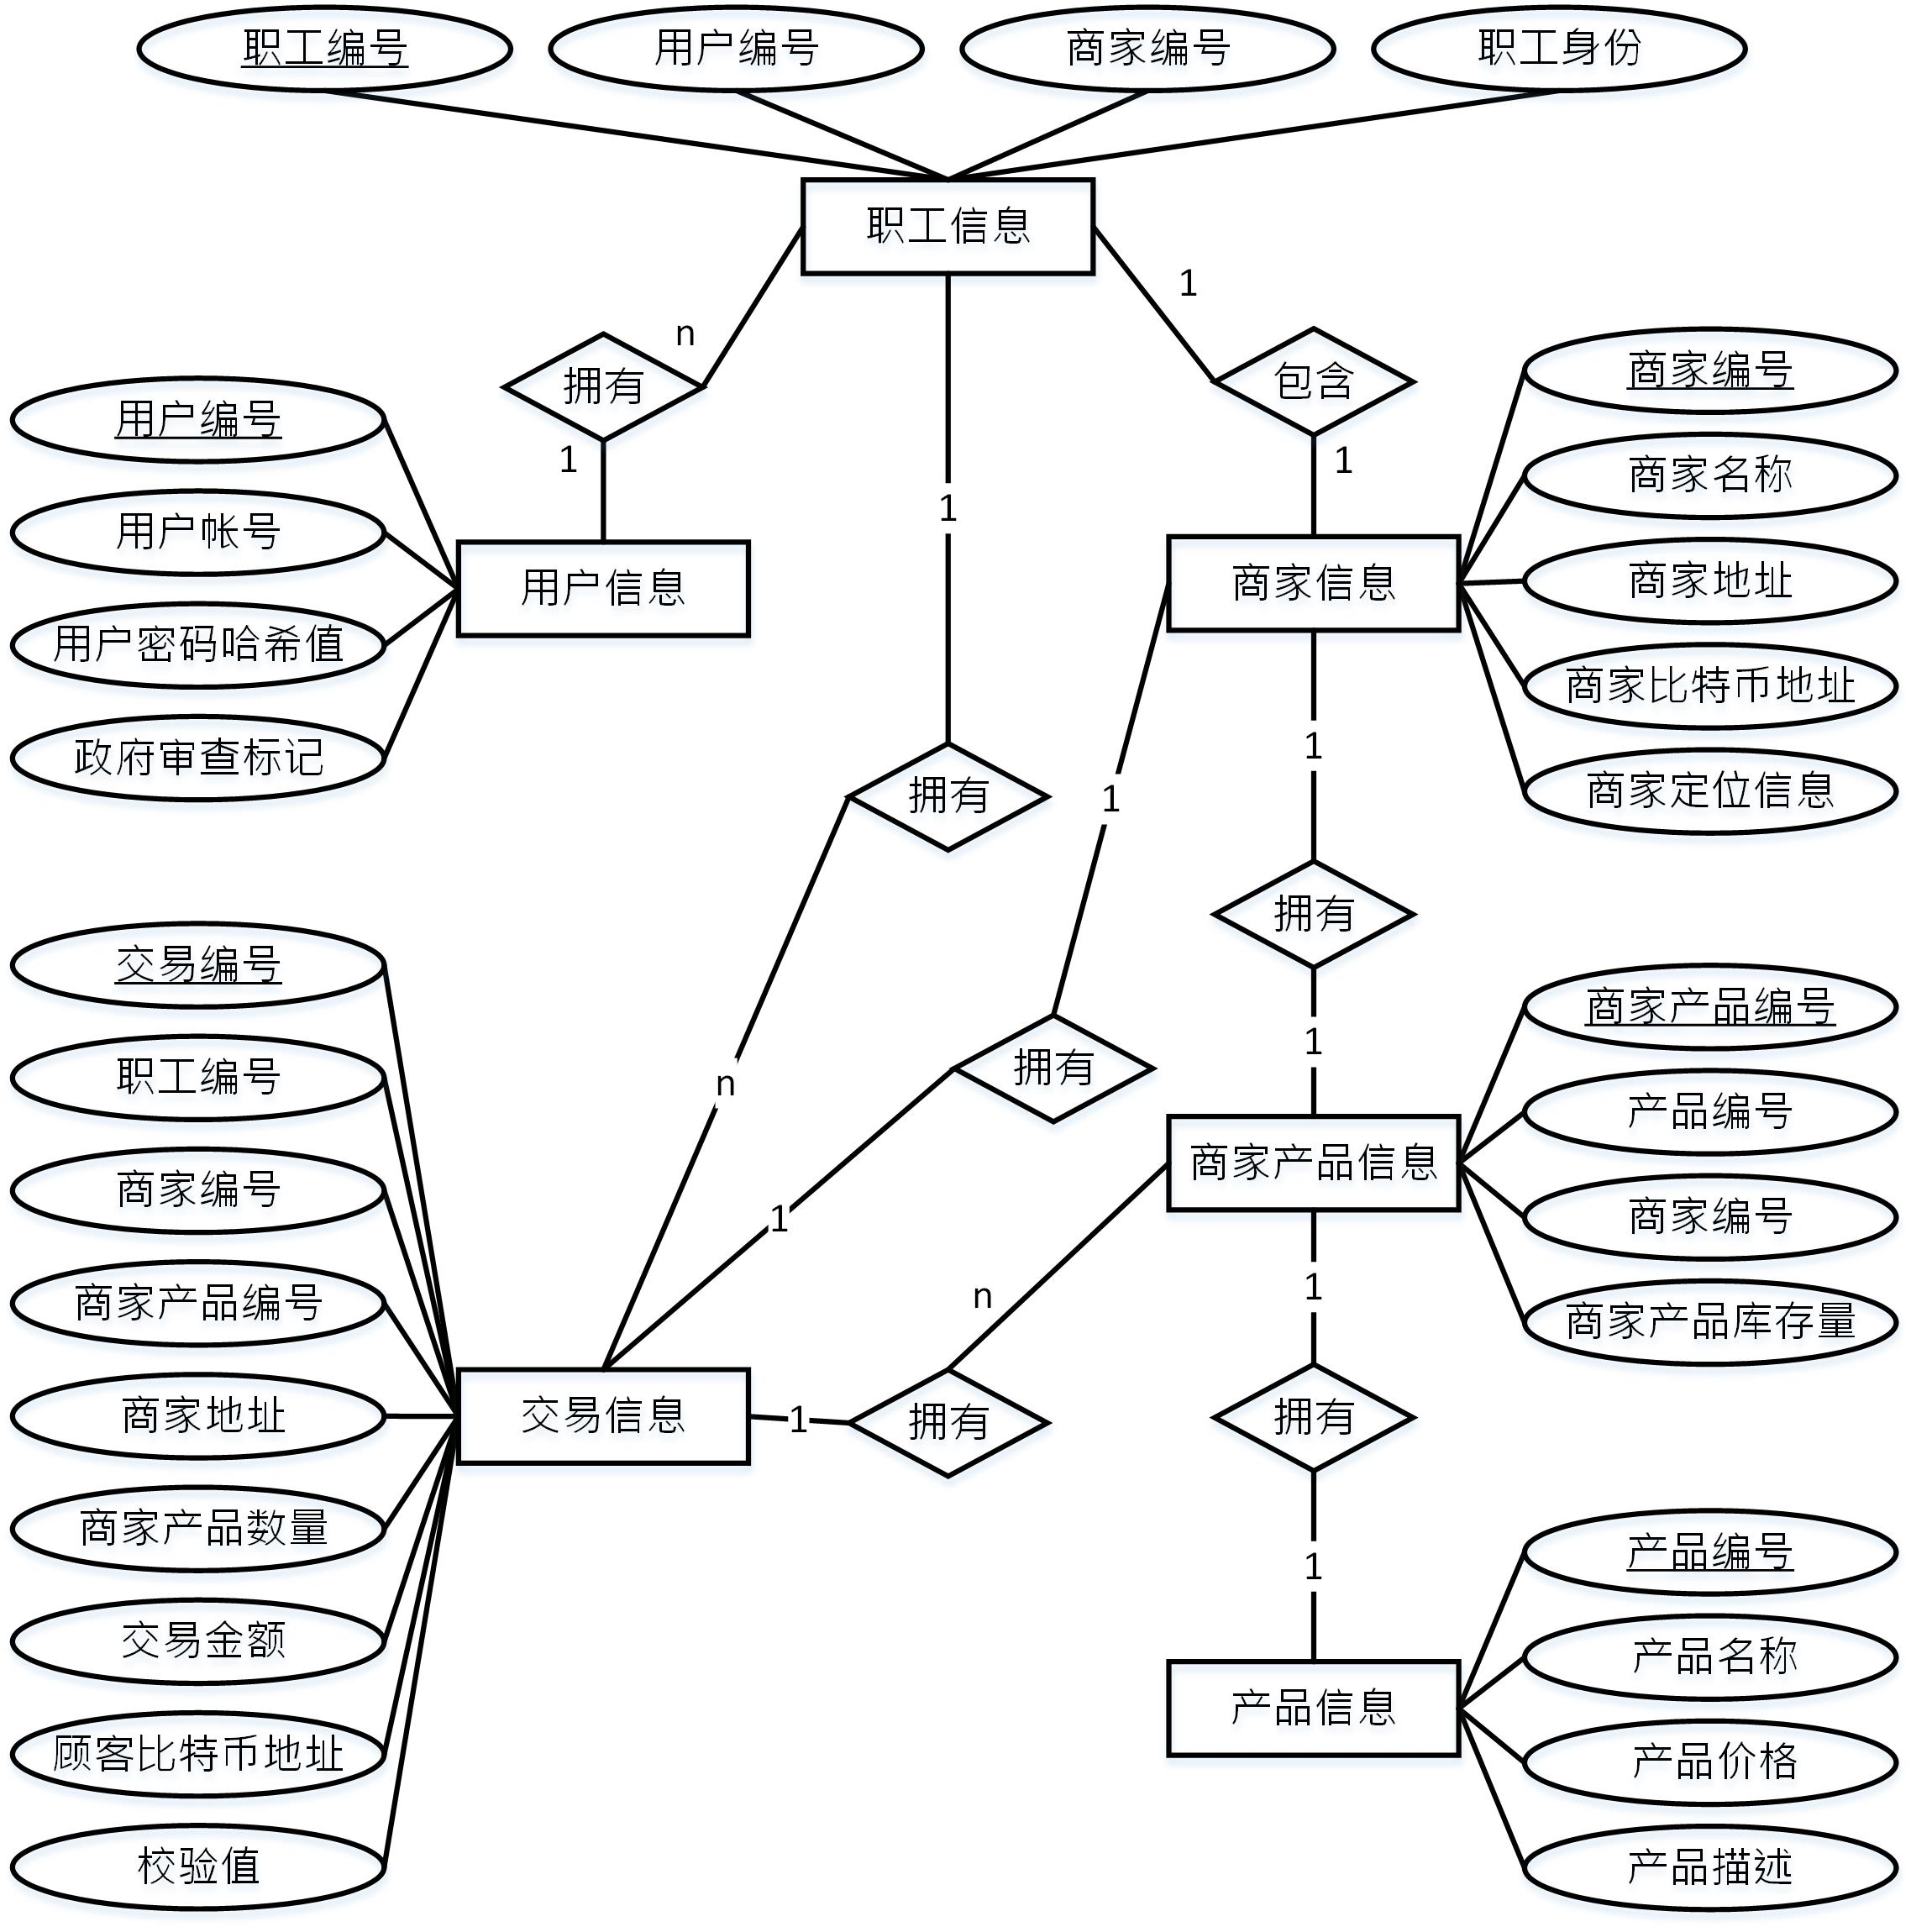
\includegraphics[width = 1\textwidth]{er.jpg}
			\caption{BRTMS數據庫實體關係圖}\label{db}
		\end{figure}

		\begin{enumerate}
		\item 商家信息表:存儲正在審核中的企業信息或已經過審核的企業信息。表\ref{store}存儲的信息包括商家編號、商家名稱、商家地址、商家比特幣地址以及商家定位信息。


				\begin{table}[htbp]
				\centering
				\caption{商家信息表}
				\label{store}
				\resizebox{\textwidth}{!}{%
				\begin{tabular}{|c|c|c|c|c|c|}
				\hline
				序號 & 字段名 & 字段說明 & 類型 & 是否為空 & 主外鍵 \\ \hline
				1 & STORE\_ID & 商家編號 & int & 否 & PK \\ \hline
				2 & STORE\_NAME & 商家名稱 & navarchar(20) & 否 &  \\ \hline
				3 & STORE\_ADDRESS & 商家地址 & navarchar(50) & 否 &  \\ \hline
				4 & STORE\_BTCADDRESS & 商家比特幣地址 & navarchar(50) & 否 &  \\ \hline
				5 & STORE\_GPS & 商家定位信息 & navarchar(30) & 否 &  \\ \hline
				\end{tabular}%
				}
				\end{table}

		\item 產品信息表:只有授權用戶才能登錄添加或修改交易產品信息。表\ref{product}產品信息表內容包括產品編號、產品名稱、產品價格以及產品描述信息。

				\begin{table}[htbp]
				\centering
				\caption{產品信息表}
				\label{product}
				
				\begin{tabular}{|c|c|c|c|c|c|}
				\hline
				序號 & 字段名 & 字段說明 & 類型 & 是否為空 & 主外鍵 \\ \hline
				1 & PRODUCT\_ID & 產品編號 & int & 否 & PK \\ \hline
				2 & PRODUCT\_NAME & 產品名稱 & navarchar(10) & 否 &  \\ \hline
				3 & PRODUCT\_PRICE & 產品價格 & float & 否 &  \\ \hline
				4 & PRODUCT\_DESCRIPTION & 產品描述 & navarchar(50) & 是 &  \\ \hline
				\end{tabular}
				\end{table}

		\item 交易信息表:表\ref{tx}記錄包括交易編號、職工編號、商家編號、商家產品編號、商家地址、商家產品數量、交易金額、顧客比特幣地址和最後確認字段的值。

				% \usepackage{graphicx}
				\begin{table}[htbp]
				\centering
				\caption{交易信息表}
				\label{tx}
				\resizebox{\textwidth}{!}{%
				\begin{tabular}{|c|c|c|c|c|c|}
				\hline
				序號 & 字段名 & 字段說明 & 類型 & 是否為空 & 主外鍵 \\ \hline
				1 & TX\_ID & 交易編號 & int & 否 & PK \\ \hline
				2 & STAFF\_ID & 職工編號 & int & 否 & FK \\ \hline
				3 & STORE\_ID & 商家編號 & int & 否 & FK \\ \hline
				4 & STOREPRODUCT\_ID & 商家產品編號 & int & 否 & FK \\ \hline
				5 & STORE\_ADDRESS & 商家地址 & navarchar(50) & 否 & FK \\ \hline
				6 & STOREPRODUCT\_QUANTITY & 商家產品數量 & int & 否 &  \\ \hline
				7 & TX\_AMOUNT & 交易金額 & float & 否 &  \\ \hline
				8 & CONSUMER\_BTCADDRESS & 顧客比特幣地址 & navarchar(50) & 否 &  \\ \hline
				9 & CHEK & 校驗值 & bool & 否 &  \\ \hline
				\end{tabular}%
				}
				\end{table}

		\item 用戶信息表:表\ref{user}存儲所有使用者信息,包括政府、商家及顧客之個人的帳戶編號與帳號,而使用者密碼則以哈希值的方式保存以增加用戶安全性。

				\begin{table}[htbp]
				\centering
				\caption{用戶信息表}
				\label{user}
				\resizebox{\textwidth}{!}{%
				\begin{tabular}{|c|c|c|c|c|c|}
				\hline
				序號 & 字段名 & 字段說明 & 類型 & 是否為空 & 主外鍵 \\ \hline
				1 & USER\_ID & 用戶編號 & int & 否 & PK \\ \hline
				2 & USER\_ACCOUNT & 用戶帳號 & navarchar(30) & 否 &  \\ \hline
				3 & USER\_PASSWORDHASH & 用戶密碼哈希值 & navarchar(30) & 否 &  \\ \hline
				4 & GOVT\_AUTH & 政府審查 & bool & 否 &  \\ \hline
				\end{tabular}
				}
				\end{table}

		\item 職工信息表:表\ref{staff}信息表存儲各個商家擁有的職工信息,包括各職工編號、用戶編號商家編號及職工身份。
				\begin{table}[htbp]
				\centering
				\caption{職工信息表}
				\label{staff}
				\begin{tabular}{|c|c|c|c|c|c|}
				\hline
				序號 & 字段名 & 字段說明 & 類型 & 是否為空 & 主外鍵 \\ \hline
				1 & STAFF\_ID & 職工編號 & int & 否 & PK \\ \hline
				2 & USER\_ID & 用戶編號 & int & 否 & FK \\ \hline
				3 & STORE\_ID & 商家編號 & int & 否 & FK \\ \hline
				4 & STAFF\_STATUS & 職工身份 & navarchar(20) & 否 &  \\ \hline
				\end{tabular}
				\end{table}

		\item 商家產品信息表:表\ref{storeproduct}存儲各家商家當前商家產品存貨信息,由商家產品編號、產品編號、商家編號及商家產品庫存量所組成。
				\begin{table}[htbp]
				\centering
				\caption{商家產品信息表}
				\label{storeproduct}
				\begin{tabular}{|c|c|c|c|c|c|}
				\hline
				序號 & 字段名 & 字段說明 & 類型 & 是否為空 & 主外鍵 \\ \hline
				1 & STOREPRODUCT\_ID & 商家產品編號 & int & 否 & PK \\ \hline
				2 & PRODUCT\_ID & 產品編號 & int & 否 & FK \\ \hline
				3 & STORE\_ID & 商家編號 & int & 否 & FK \\ \hline
				4 & STOREPRODUCT\_INVENTORY & 商家產品庫存量 & int & 否 &  \\ \hline
				\end{tabular}
				\end{table}

	\end{enumerate}

\section{系統模塊設計}
在本系統中共有三種使用者,分別為顧客、商家以及職工,首先是用戶登入與註冊模塊,其餘總共有四個管理模塊分別為商家產品管理模塊、職工管理模塊、顧客交易管理模塊和商家交易管理模塊,以下將說明各個模塊類圖設計以及時序圖運作。

\subsubsection{(一)用戶註冊與登入模塊}
在本系統中僅職工與商家需要進行註冊,並且需要經過政府的審查批准。職工與商家皆為使用者皆可使用用戶註冊模塊。

	\begin{figure}[htbp]
		\centering
		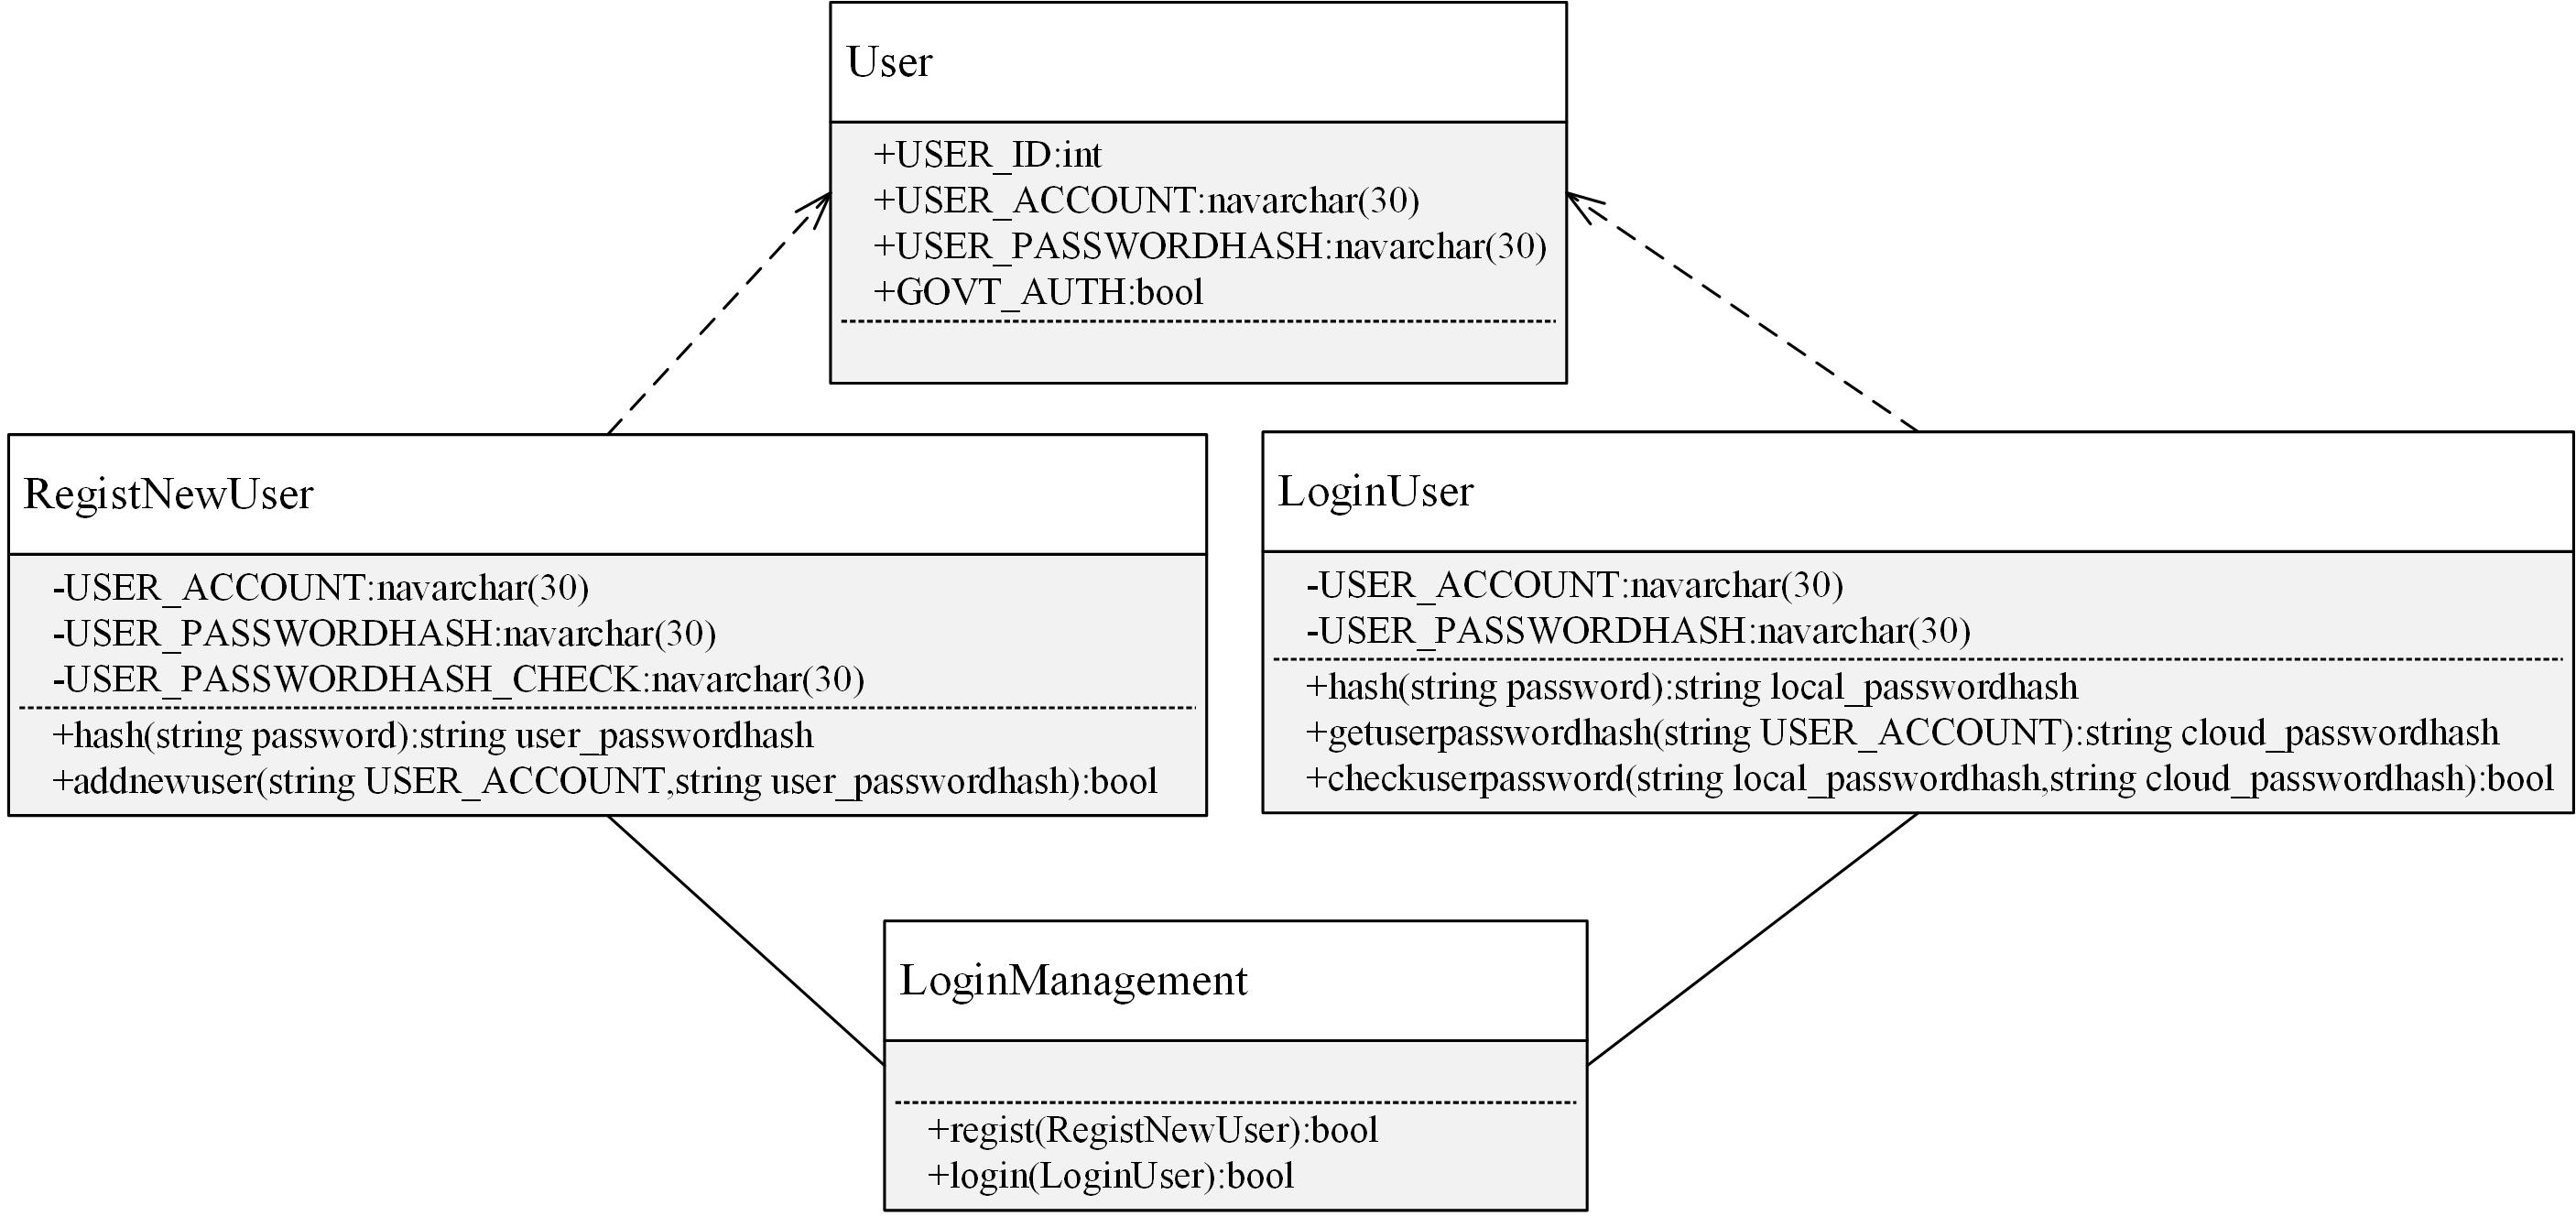
\includegraphics[width = 1\textwidth]{c3.jpg}
		\caption{用戶註冊與登入模塊類圖}\label{c3}
	\end{figure}

	圖\ref{time1}為職工與商家註冊時序圖,以下為流程說明:

	\begin{figure}[htbp]
		\centering
		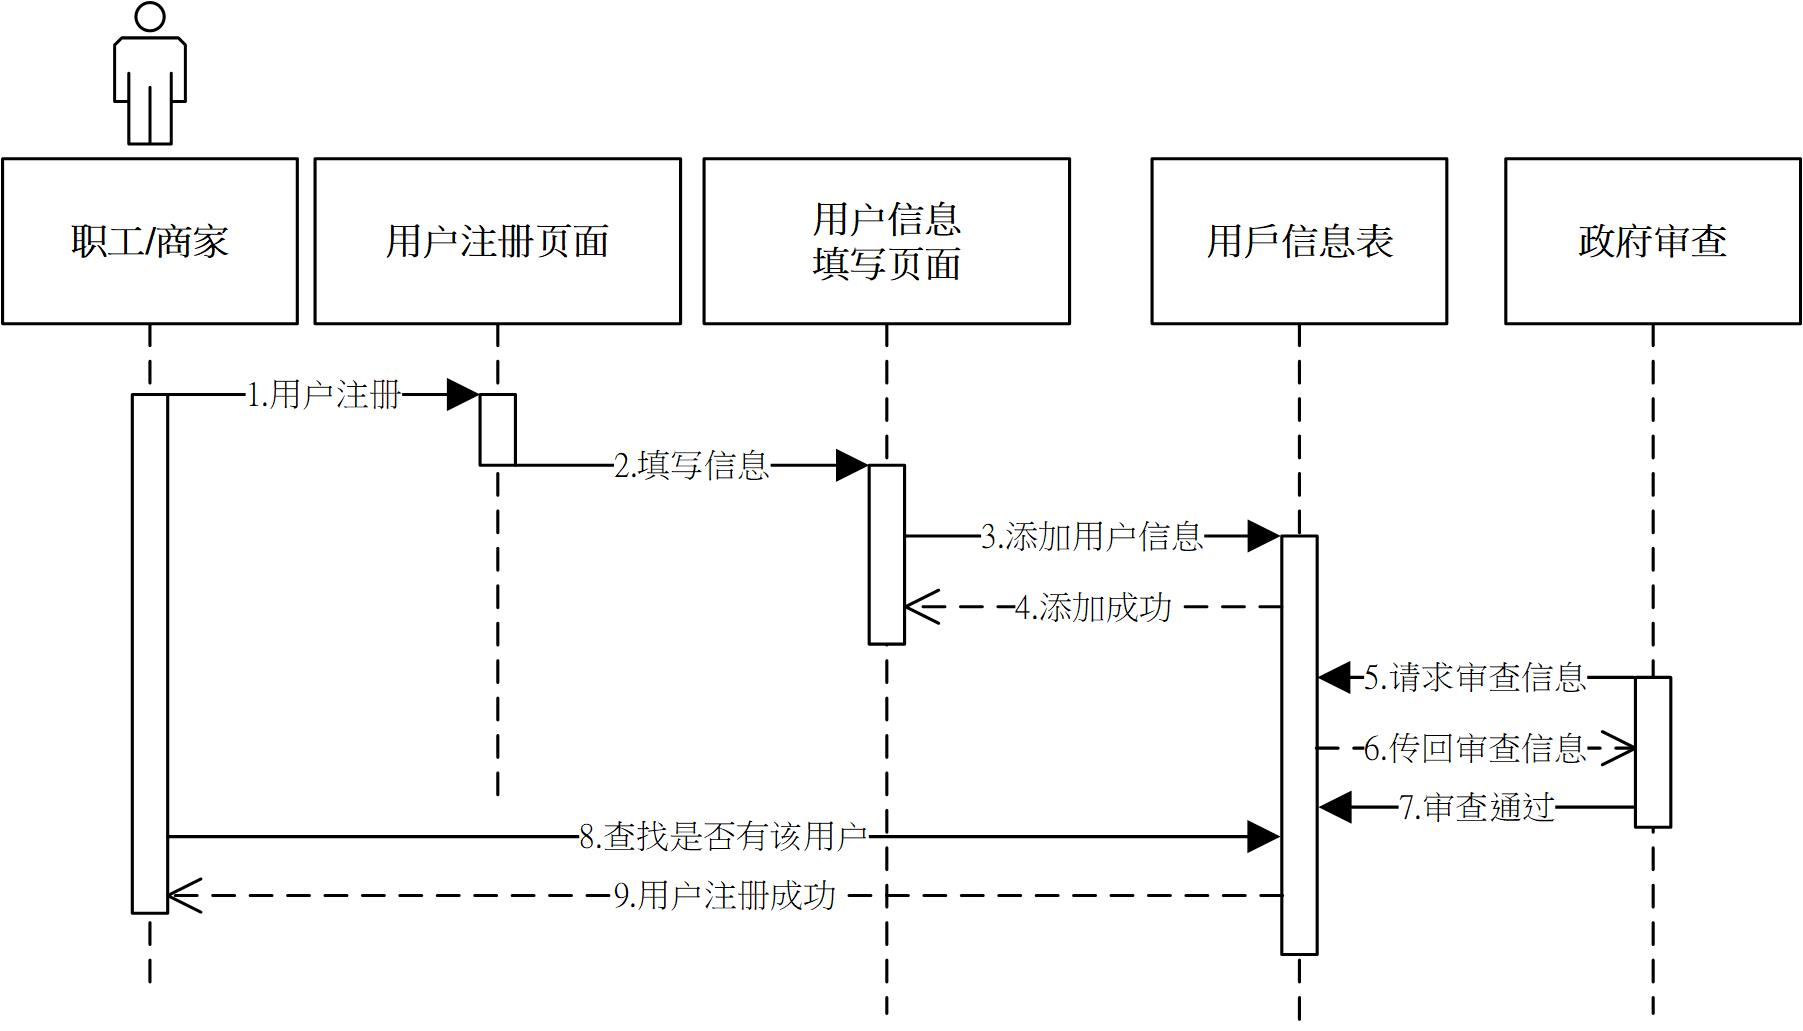
\includegraphics[width = 1\textwidth]{time1.jpg}
		\caption{職工與商家註冊時序圖}\label{time1}
	\end{figure}

	\begin{enumerate}
	\item 首先職工或是商家前往用戶註冊頁面。
	\item 前往用戶信息填寫頁面填寫用戶帳戶信息以及用戶密碼。
	\item 完成填寫後,為了提升使用者密碼信息安全,將使用者密碼以哈希算法計算後以密碼哈希值保存。將填寫完的帳號信息以及密碼哈希職提交到用戶信息表。
	\item 用戶信息表則傳為添加成功。屆時的用戶信息已經存儲到用戶信息表內但是尚未被激活,需要等待政府進行審查。
	\item 政府向用戶信息請求表拿取所有還未被激活的用戶信息。
	\item 數據庫中的用戶信息表傳回,政府請求的用戶信息清單。
	\item 政府進行用戶審查,在完成用戶審查後,則向用戶信息表內輸入審查通過。
	\item 此時,用戶再次訪問用戶信息表當中,用戶帳號是否已經激活成功。
	\item 用戶信息表回傳已經驗證通過。
	\end{enumerate}


\subsubsection{(二)產品管理模塊}
商家的運營需要管理本身所需販售的商品,在商家完成註冊用戶帳號並且通過政府審核之後,便可檢視所有的產品,近一步可以透過產品管理模塊新增、修改以及刪除商家商品。

	\begin{figure}[htbp]
		\centering
		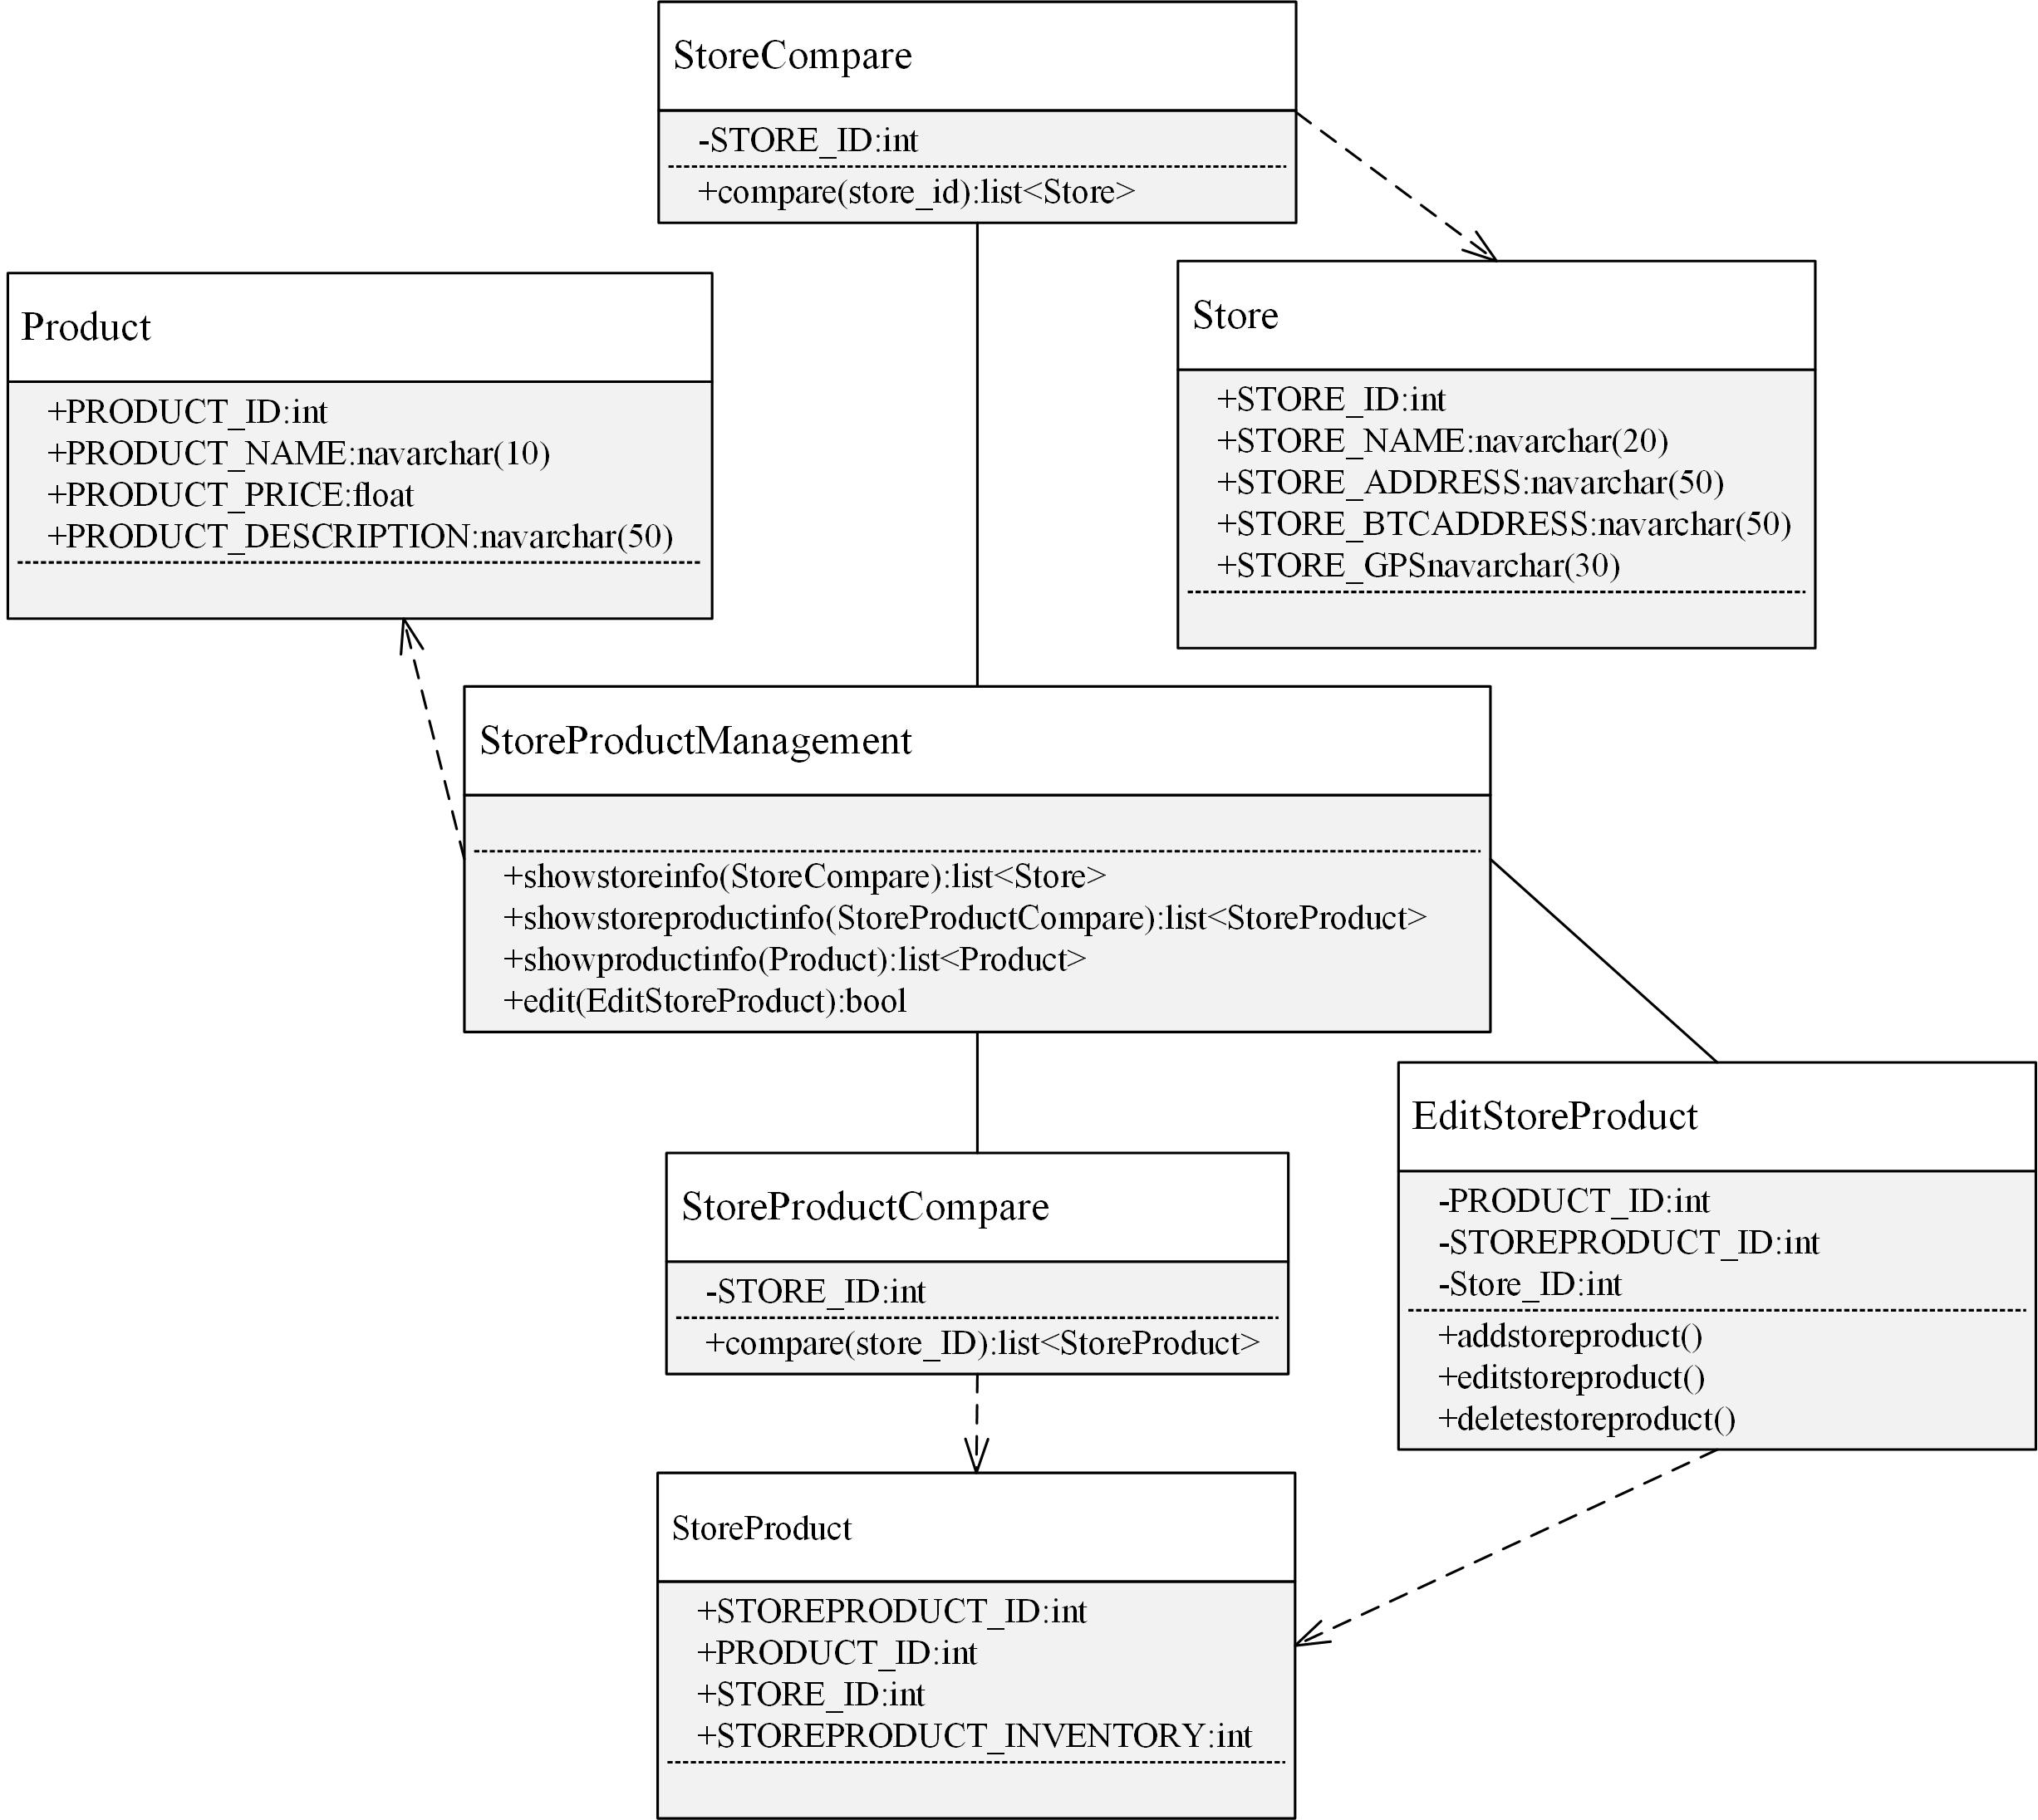
\includegraphics[width = 1\textwidth]{c2.jpg}
		\caption{商家產品管理類圖}\label{c2}
	\end{figure}

	圖\ref{time3}為商家產品管理時序圖,以下為流程說明:

	\begin{figure}[htbp]
		\centering
		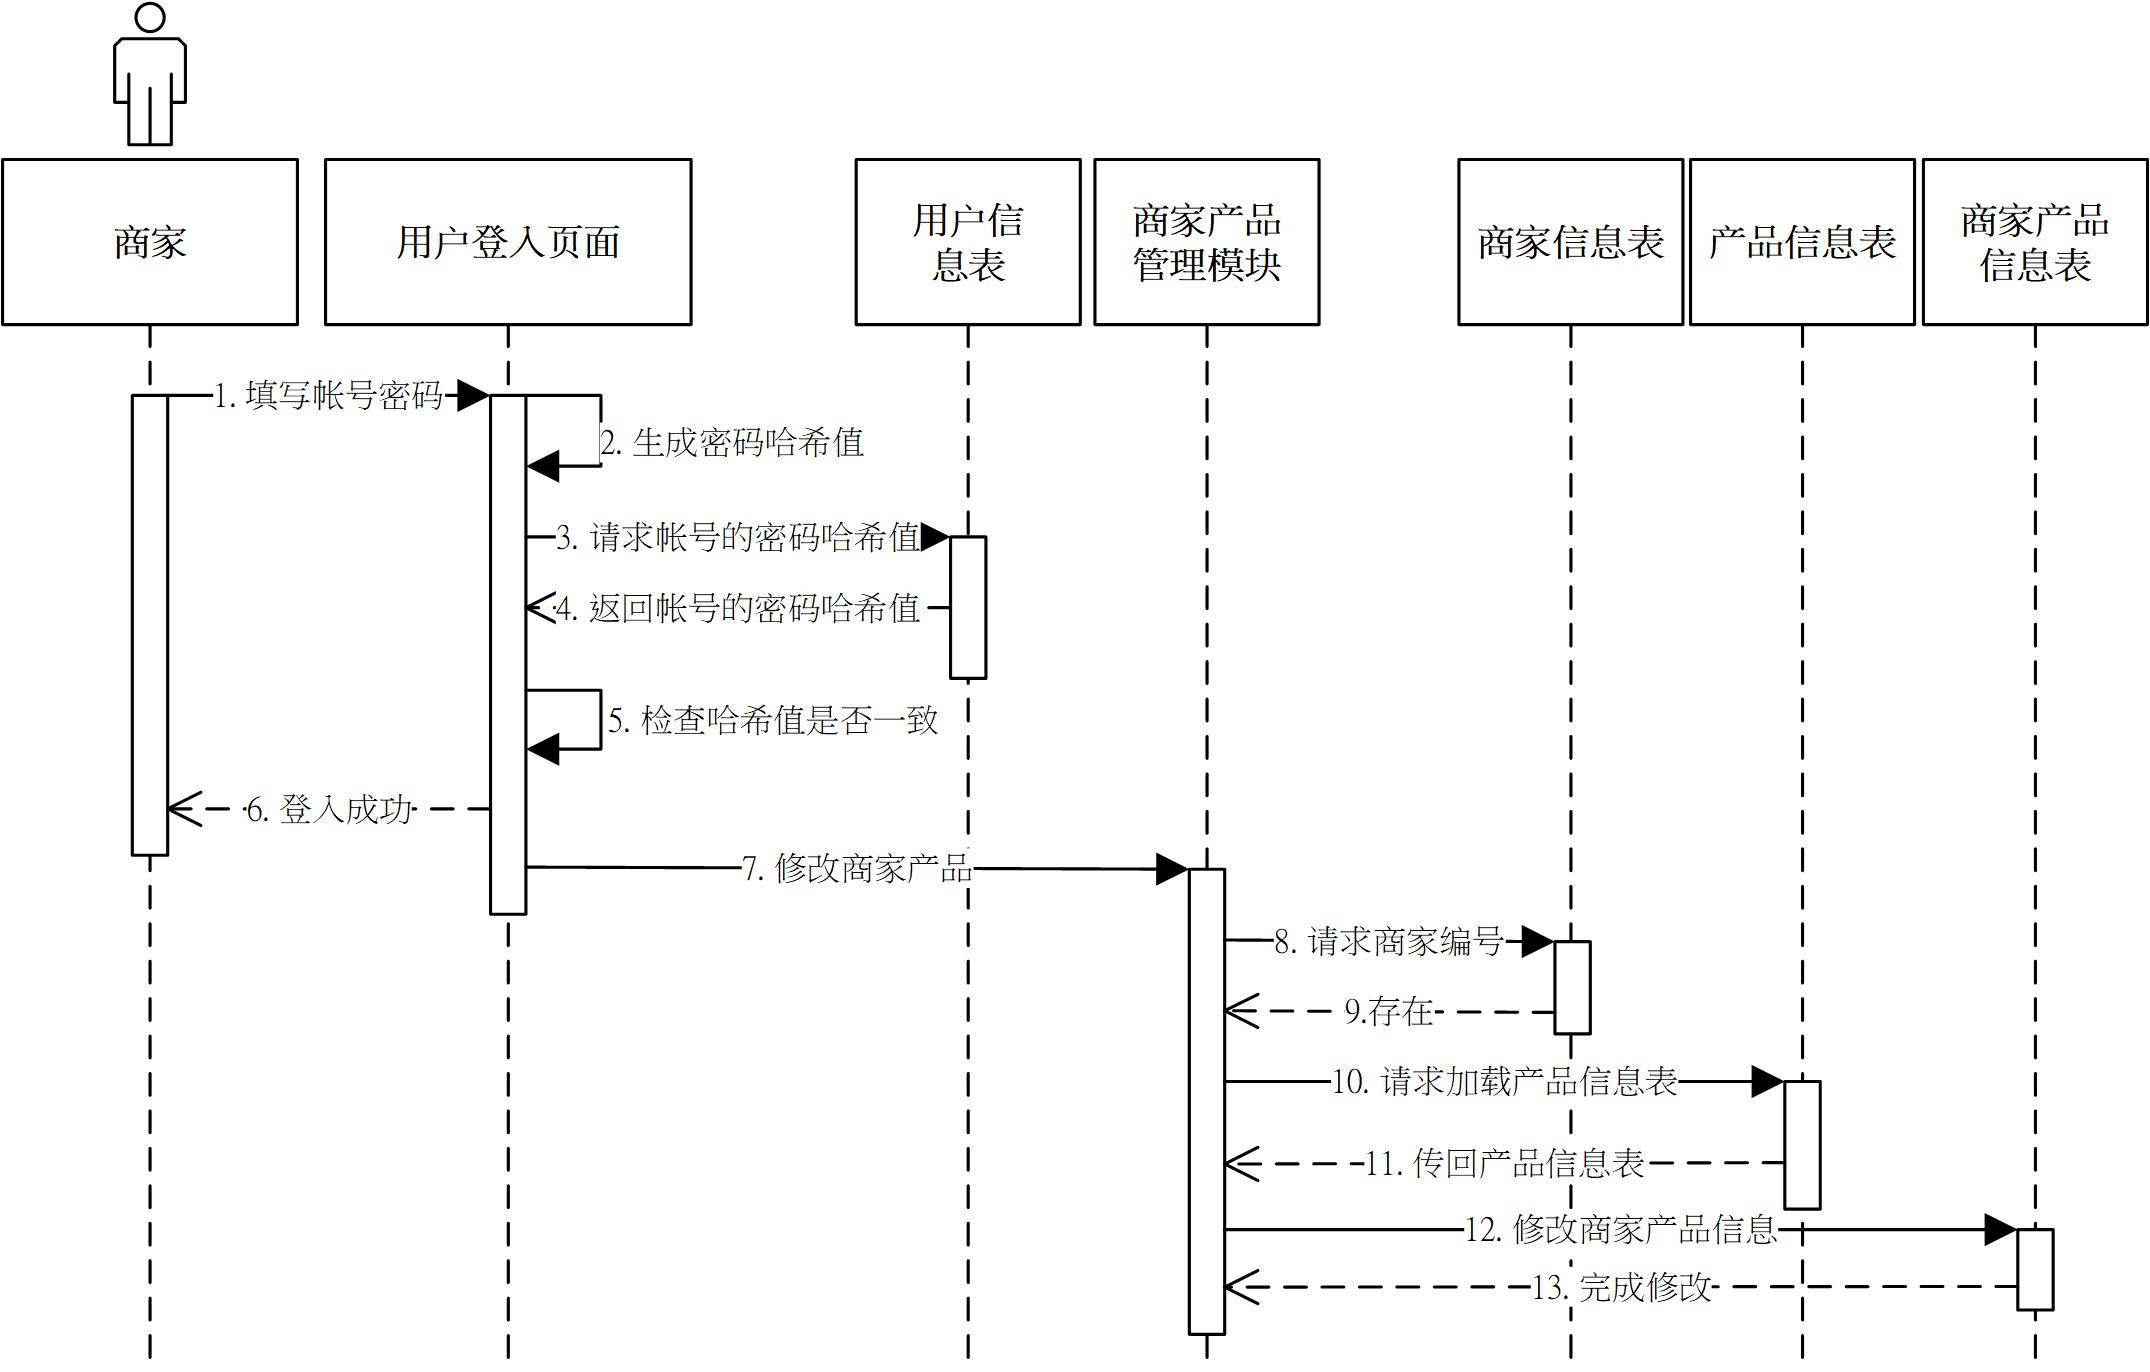
\includegraphics[width = 1\textwidth]{time3.jpg}
		\caption{商家產品管理時序圖}\label{time3}
	\end{figure}

	\begin{enumerate}
	\item 商家在完成用戶註冊後並完成政府的審核之後,便可填寫使用用戶與用戶密碼至到登入頁面。
	\item 登入頁面會將用戶提交之密碼透過哈希算法生成密碼哈希值。
	\item 用戶登入頁面向用戶信息表詢問該用戶帳號的密碼哈希值。
	\item 用戶信息表將該帳戶的密碼哈希值傳回給用戶登入頁面保存。
	\item 用戶頁面將本地密碼哈希值和從數據庫信息表中請求保存的密碼哈希值進行比對是否相同。
	\item 倘若本地與數據庫中的哈希值一至,則為都入成功。
	\item 屆時可以進入商家產品管理模塊。
	\item 為確認預修改的商家是否存在,所以向數據庫中的商家信息表請求該商家編號是否存在。
	\item 商家信息表返回存在的信息。
	\item 向數據庫中的產品信息表當中請求所有的產品信息。
	\item 產品信息表回傳所有的產品信息。
	\item 此時商家已經確認商家信息是否存在,且已經取得所有的產品信息。商家向商家產品信息表提交商家要增加的產品編號以及商家本身的商家編號,此時生成商家產品編號。
	\item 商家信息表在完成添加商家產品信息之後,傳回添加成功的信息到商家產品管理模塊。
	\end{enumerate}


\subsubsection{(三)職工管理模塊}
商家需要職工進行商家的運營,在商家用戶完成政府審查之後,便可以進入職工管理模塊,透過提交用戶編號以及商家編號新增、修改以及刪除職工信息。

	\begin{figure}[htbp]
		\centering
		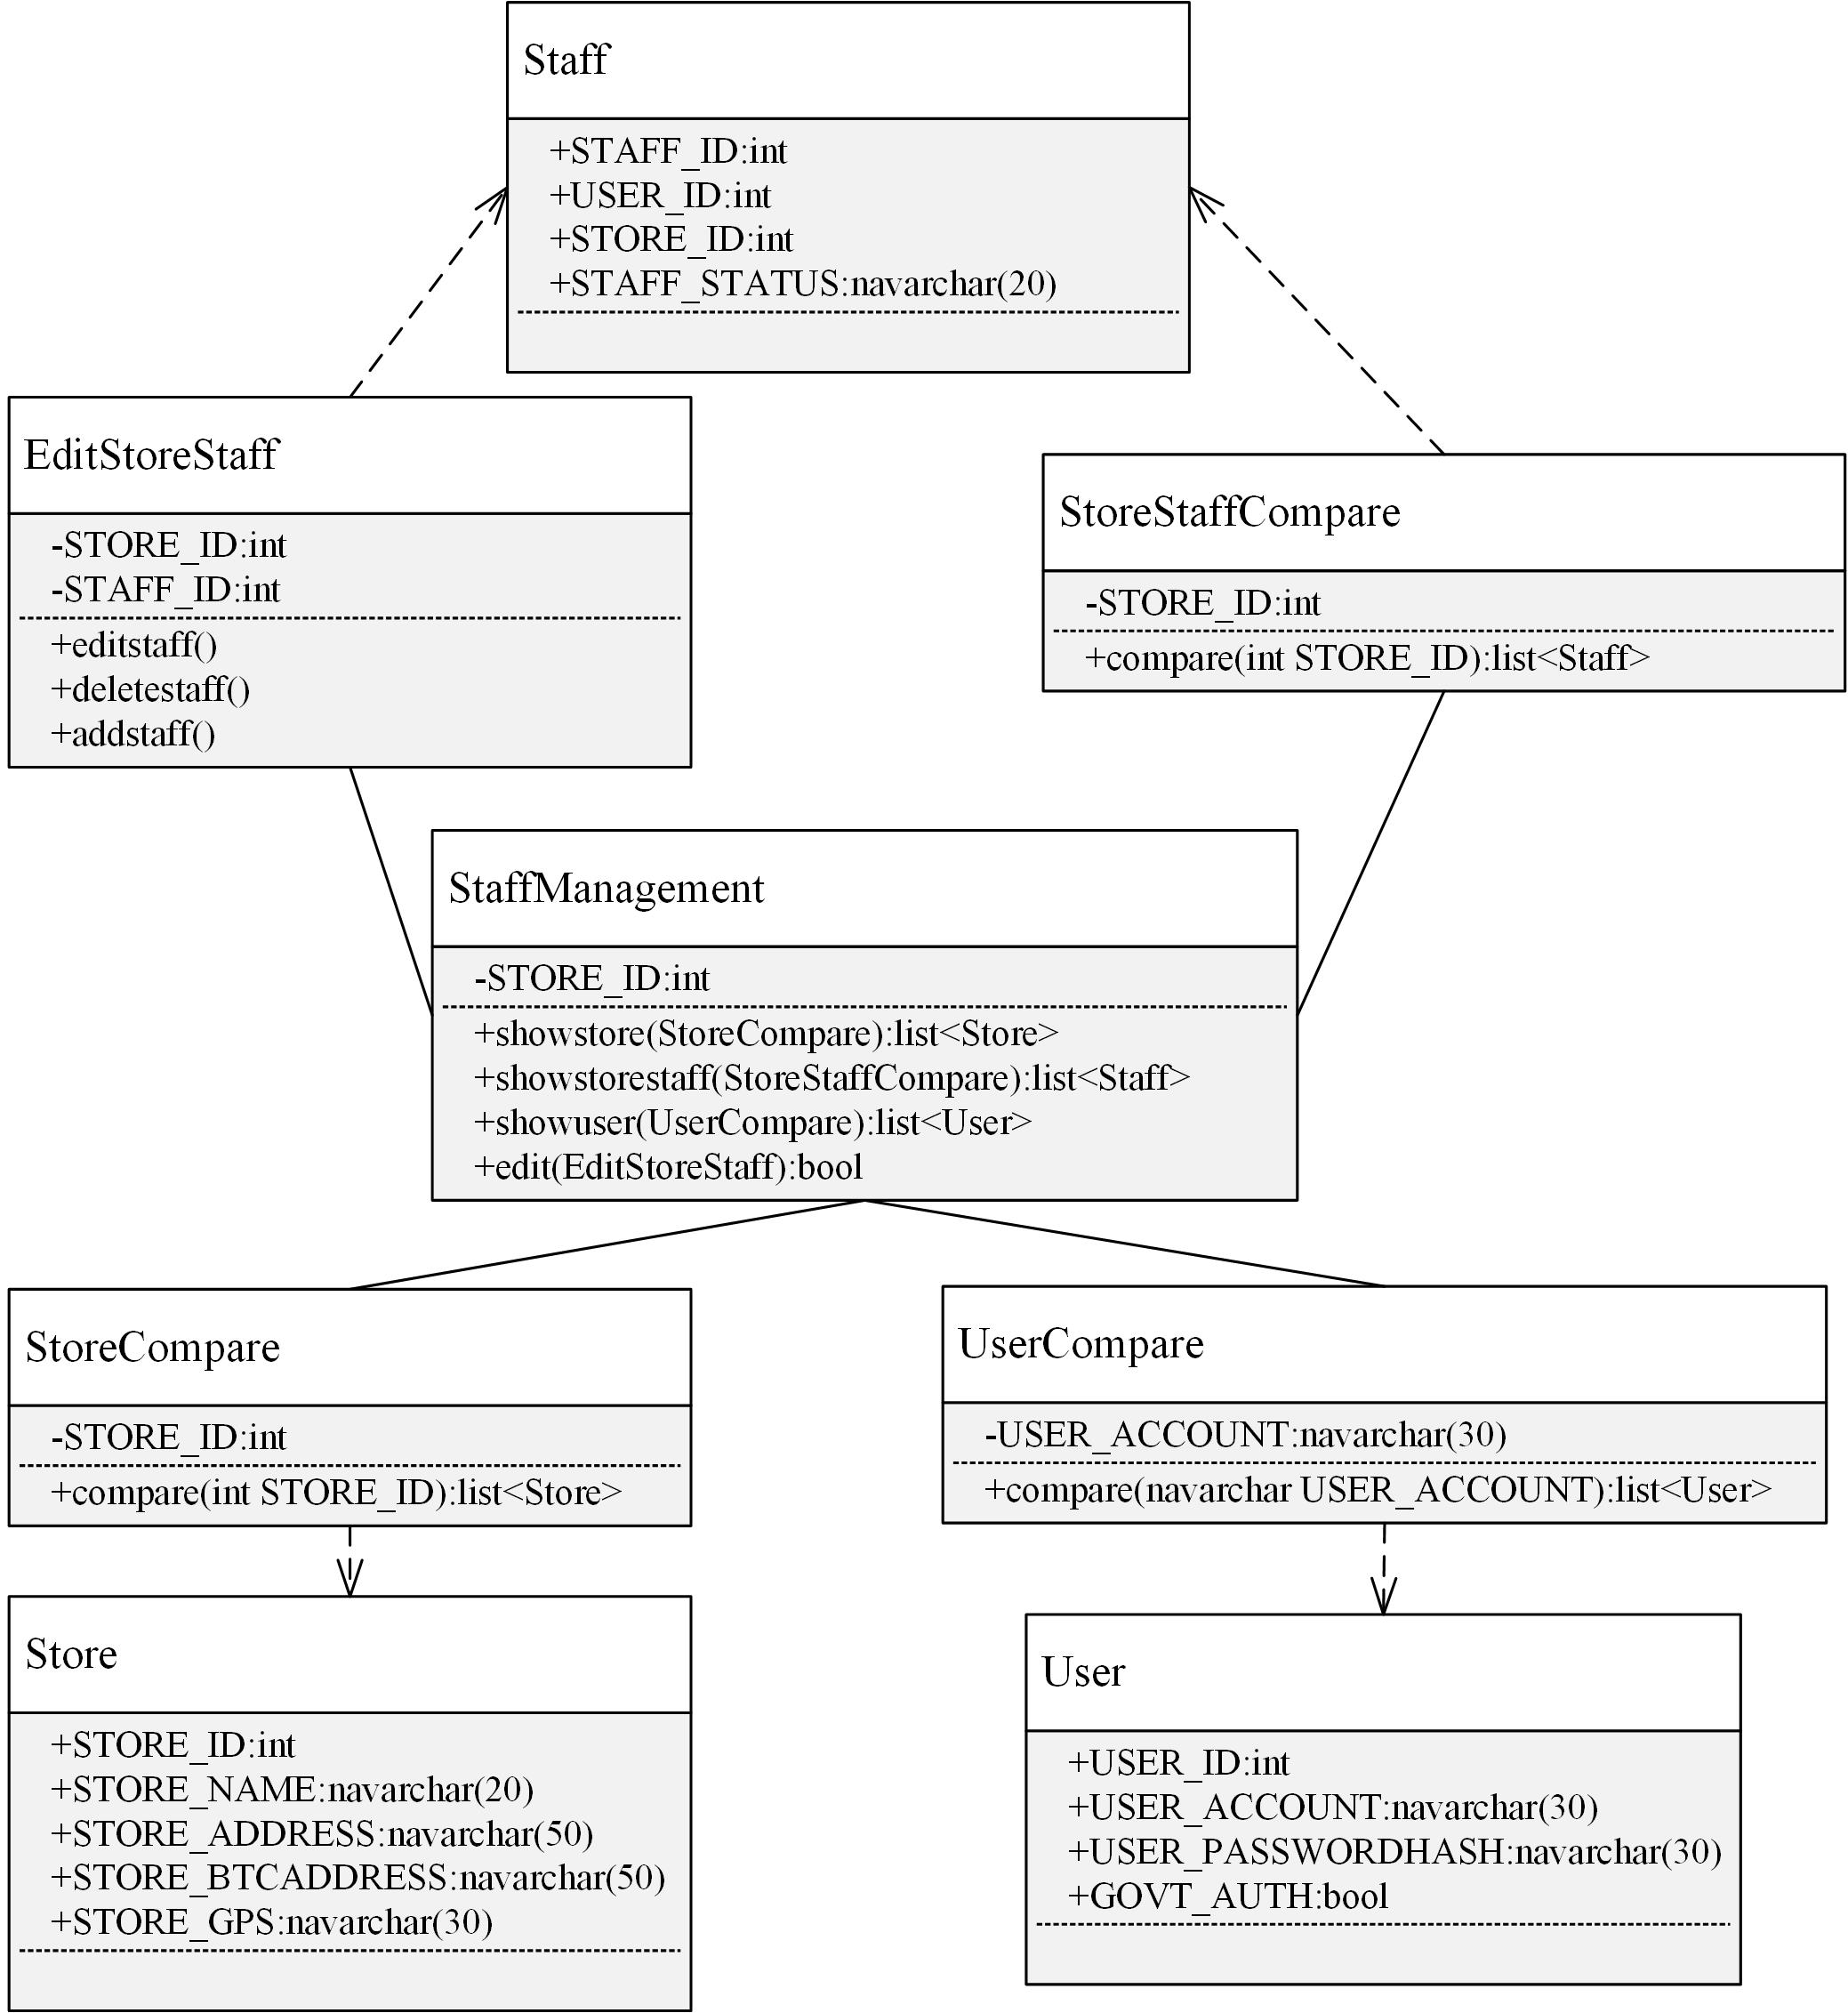
\includegraphics[width = 1\textwidth]{c1.jpg}
		\caption{職工管理模塊類圖}\label{c1}
	\end{figure}

	

	圖\ref{time2}為商家職工管理時序圖,以下為流程說明:

	\begin{figure}[htbp]
		\centering
		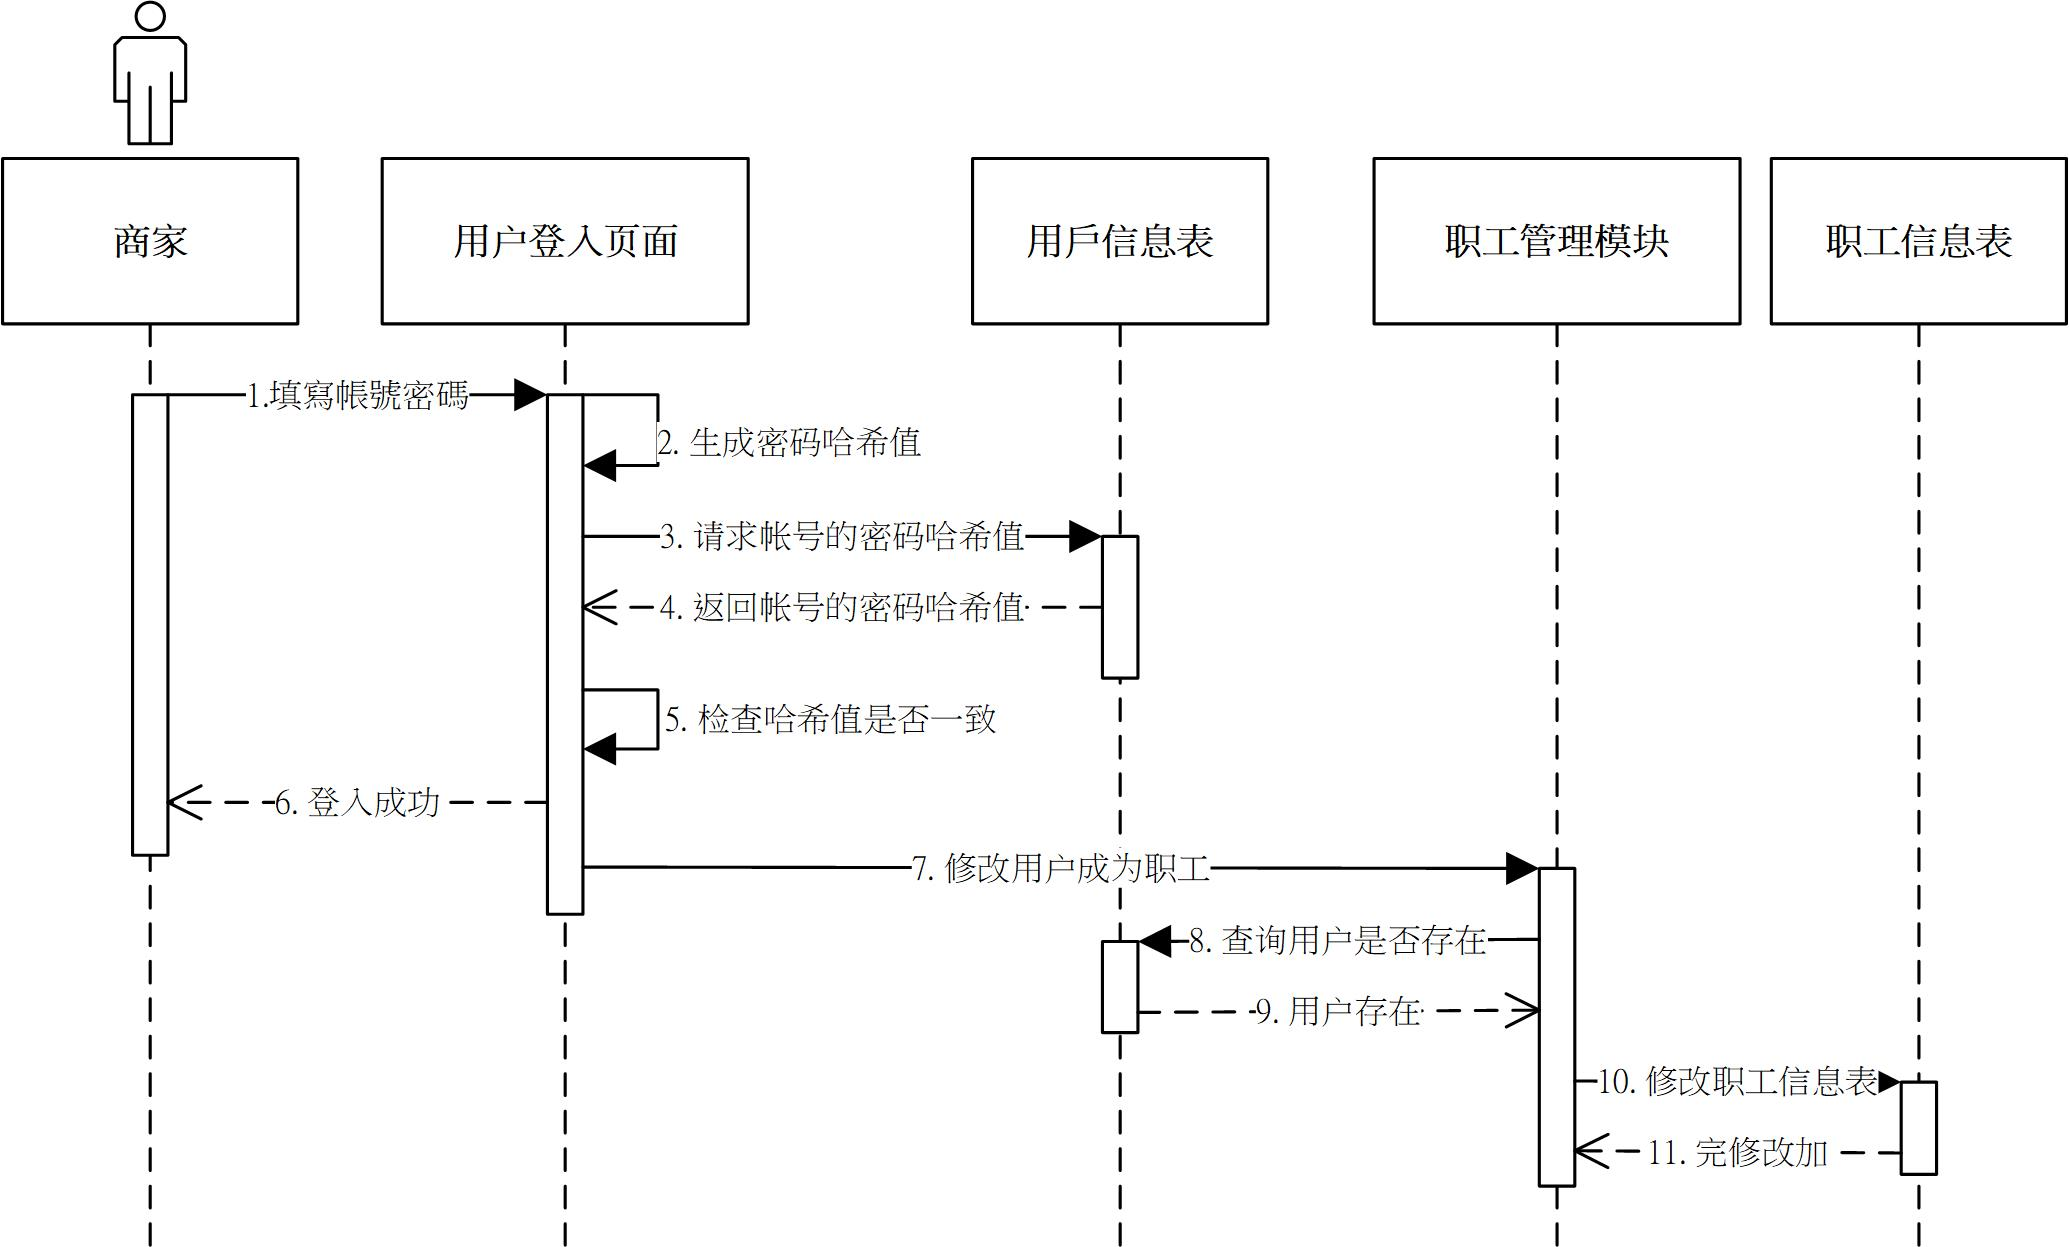
\includegraphics[width = 1\textwidth]{time2.jpg}
		\caption{商家職工管理時序圖}\label{time2}
	\end{figure}

	\begin{enumerate}
	\item 商家前往用戶登入頁面輸入用戶帳號密碼。
	\item 用戶登入頁面自動使用哈希算法將用戶密碼轉換成密碼哈希值。
	\item 用戶登入頁面向數據庫中的用戶信息表請求該用戶帳號的密碼哈希值。
	\item 數據庫用戶信息表回傳用戶密碼哈希值。
	\item 用戶登入頁面比對本地端的用戶密碼哈希值與數據庫中的密碼哈希值是否一致。
	\item 倘若數據庫中的密碼哈希值與用戶登入頁面生成的密碼哈希值一致,則登入成功。
	\item 商家提交商家編號以及預添加的用戶編號。
	\item 職工管理模塊向用戶信息表查詢該用戶是否存在。
	\item 用戶信息表傳回用戶存在信息。
	\item 職工管理模塊向數據庫中的職工信息表提交用戶編號、商家編號以及職工編號修改職工信息。
	\item 職工信息表傳回修改完成。
	\end{enumerate}


\subsubsection{(四)顧客交易管理模塊}

	\begin{figure}[htbp]
		\centering
		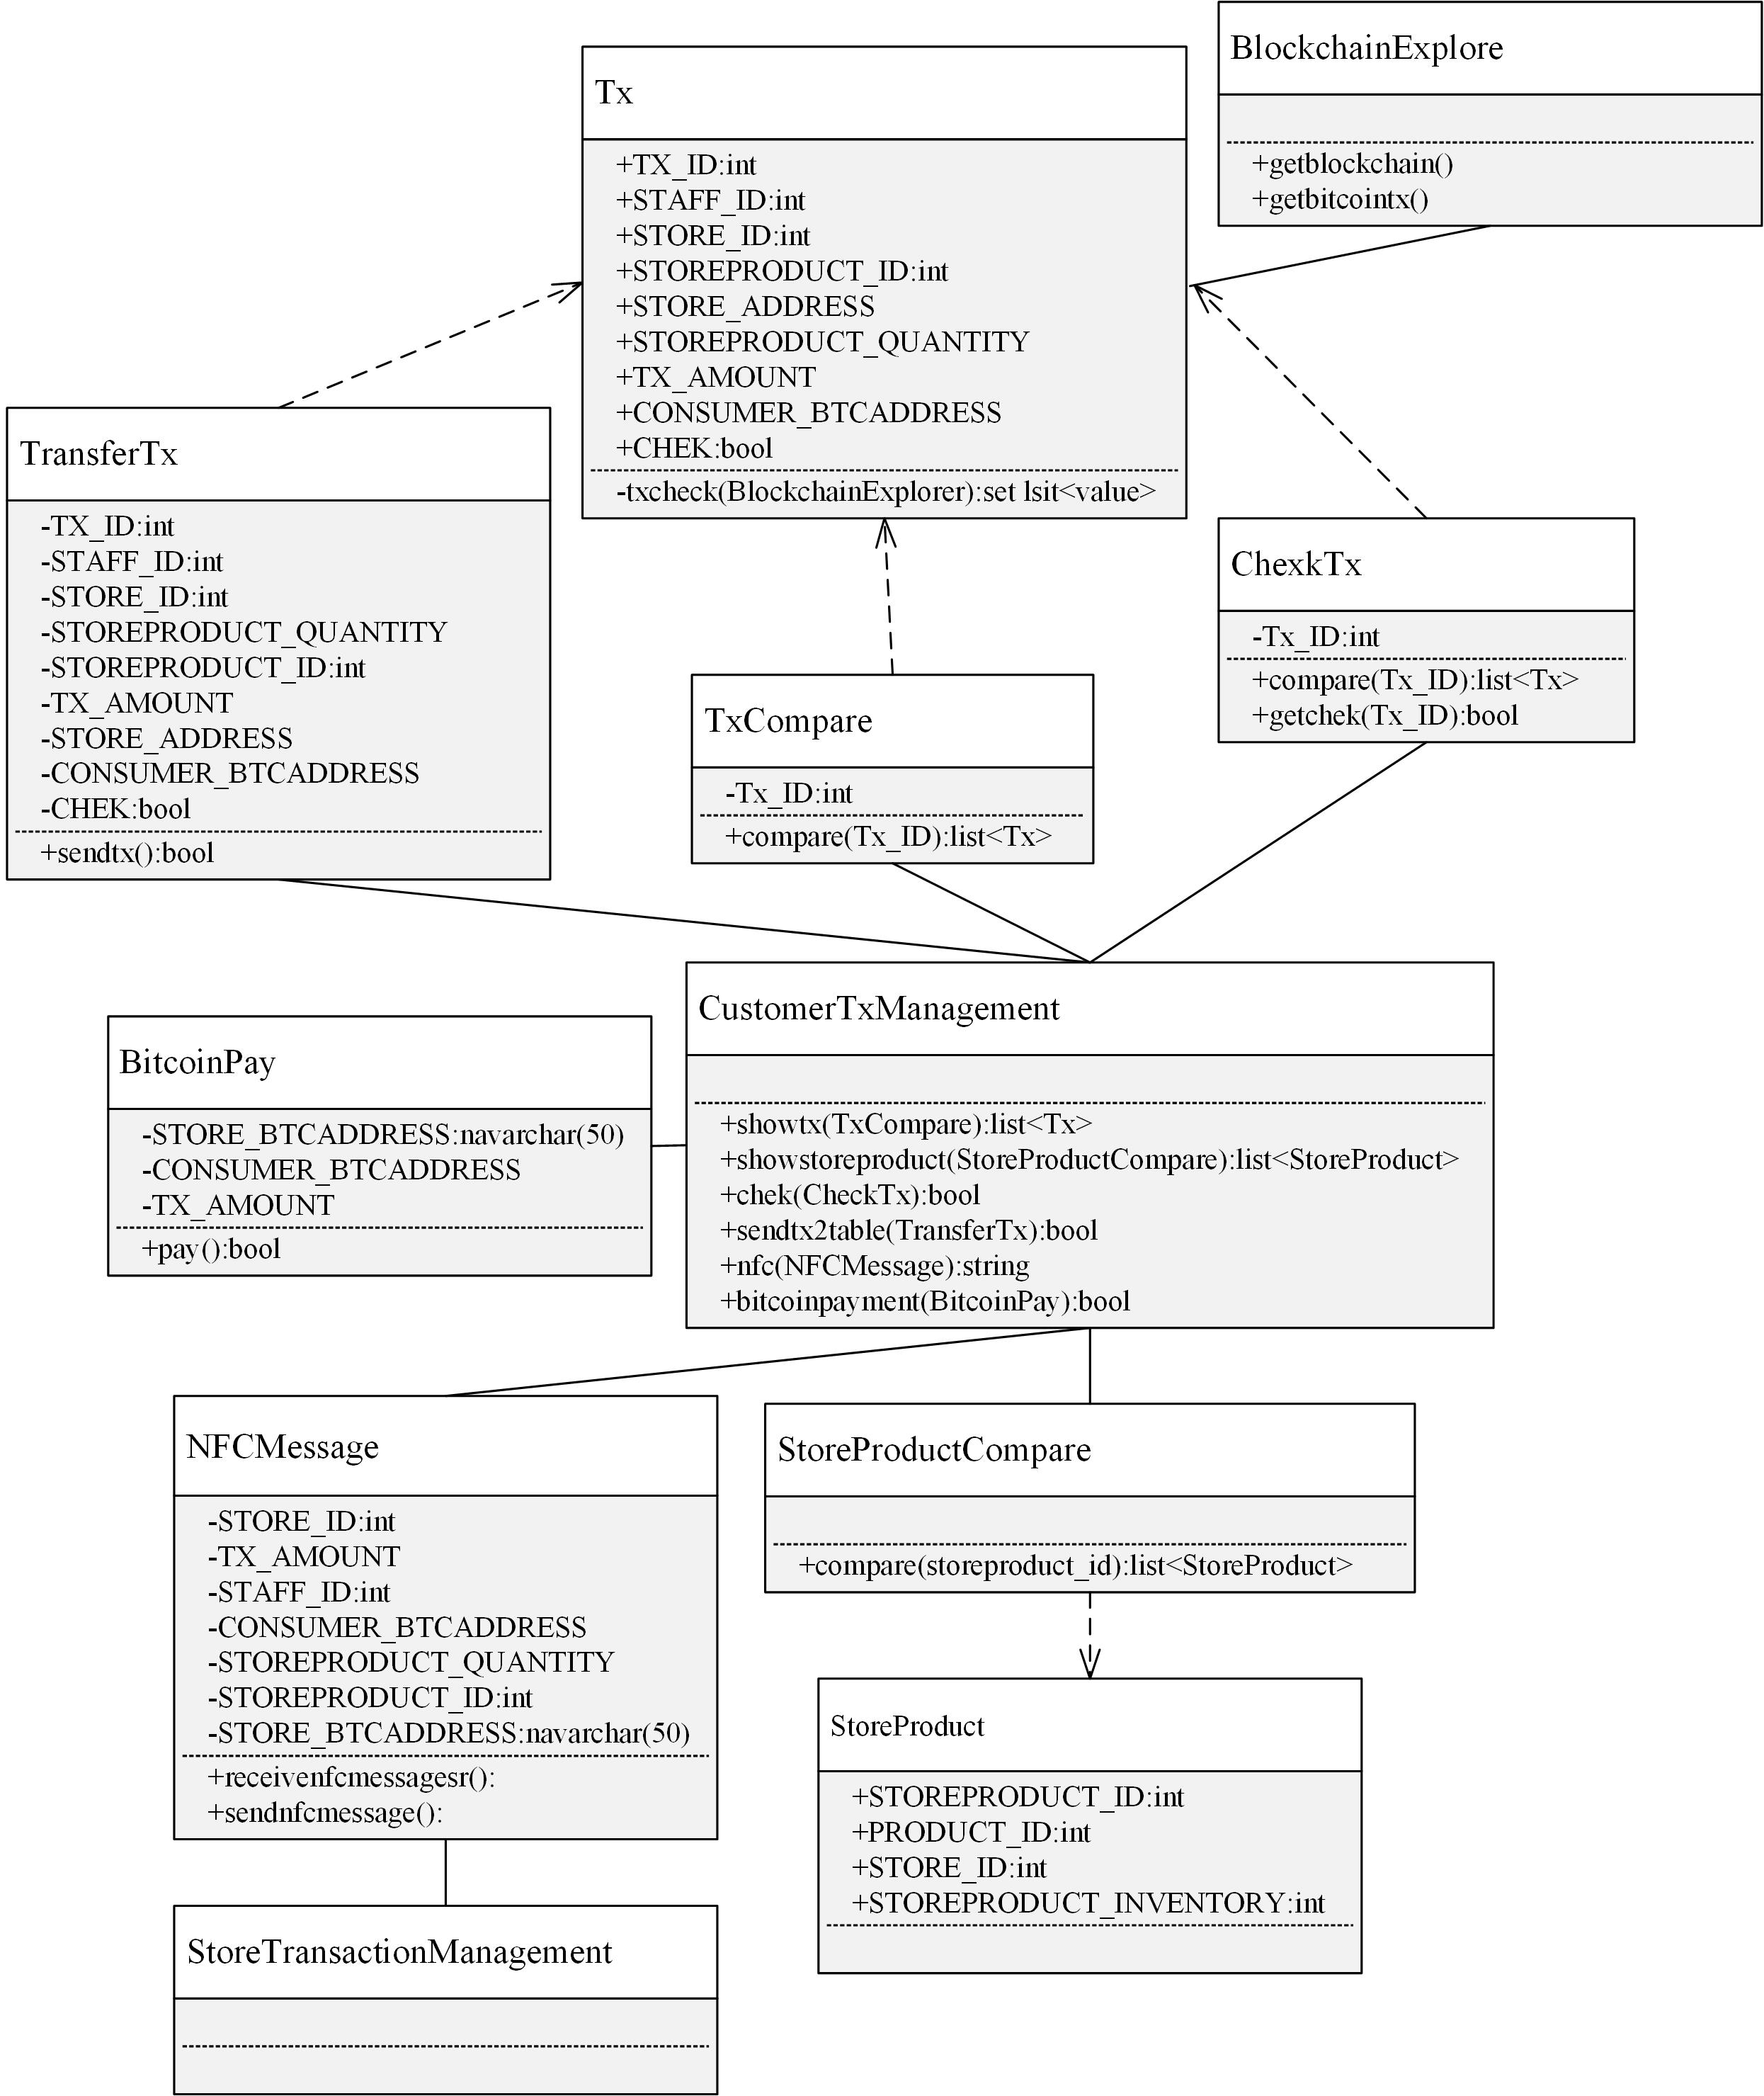
\includegraphics[width = 1\textwidth]{c4.jpg}
		\caption{顧客交易管理模塊類圖}\label{c4}
	\end{figure}

	

	圖\ref{time5}為顧客交易管理時序圖,以下為流程說明:

	\begin{figure}[htbp]
		\centering
		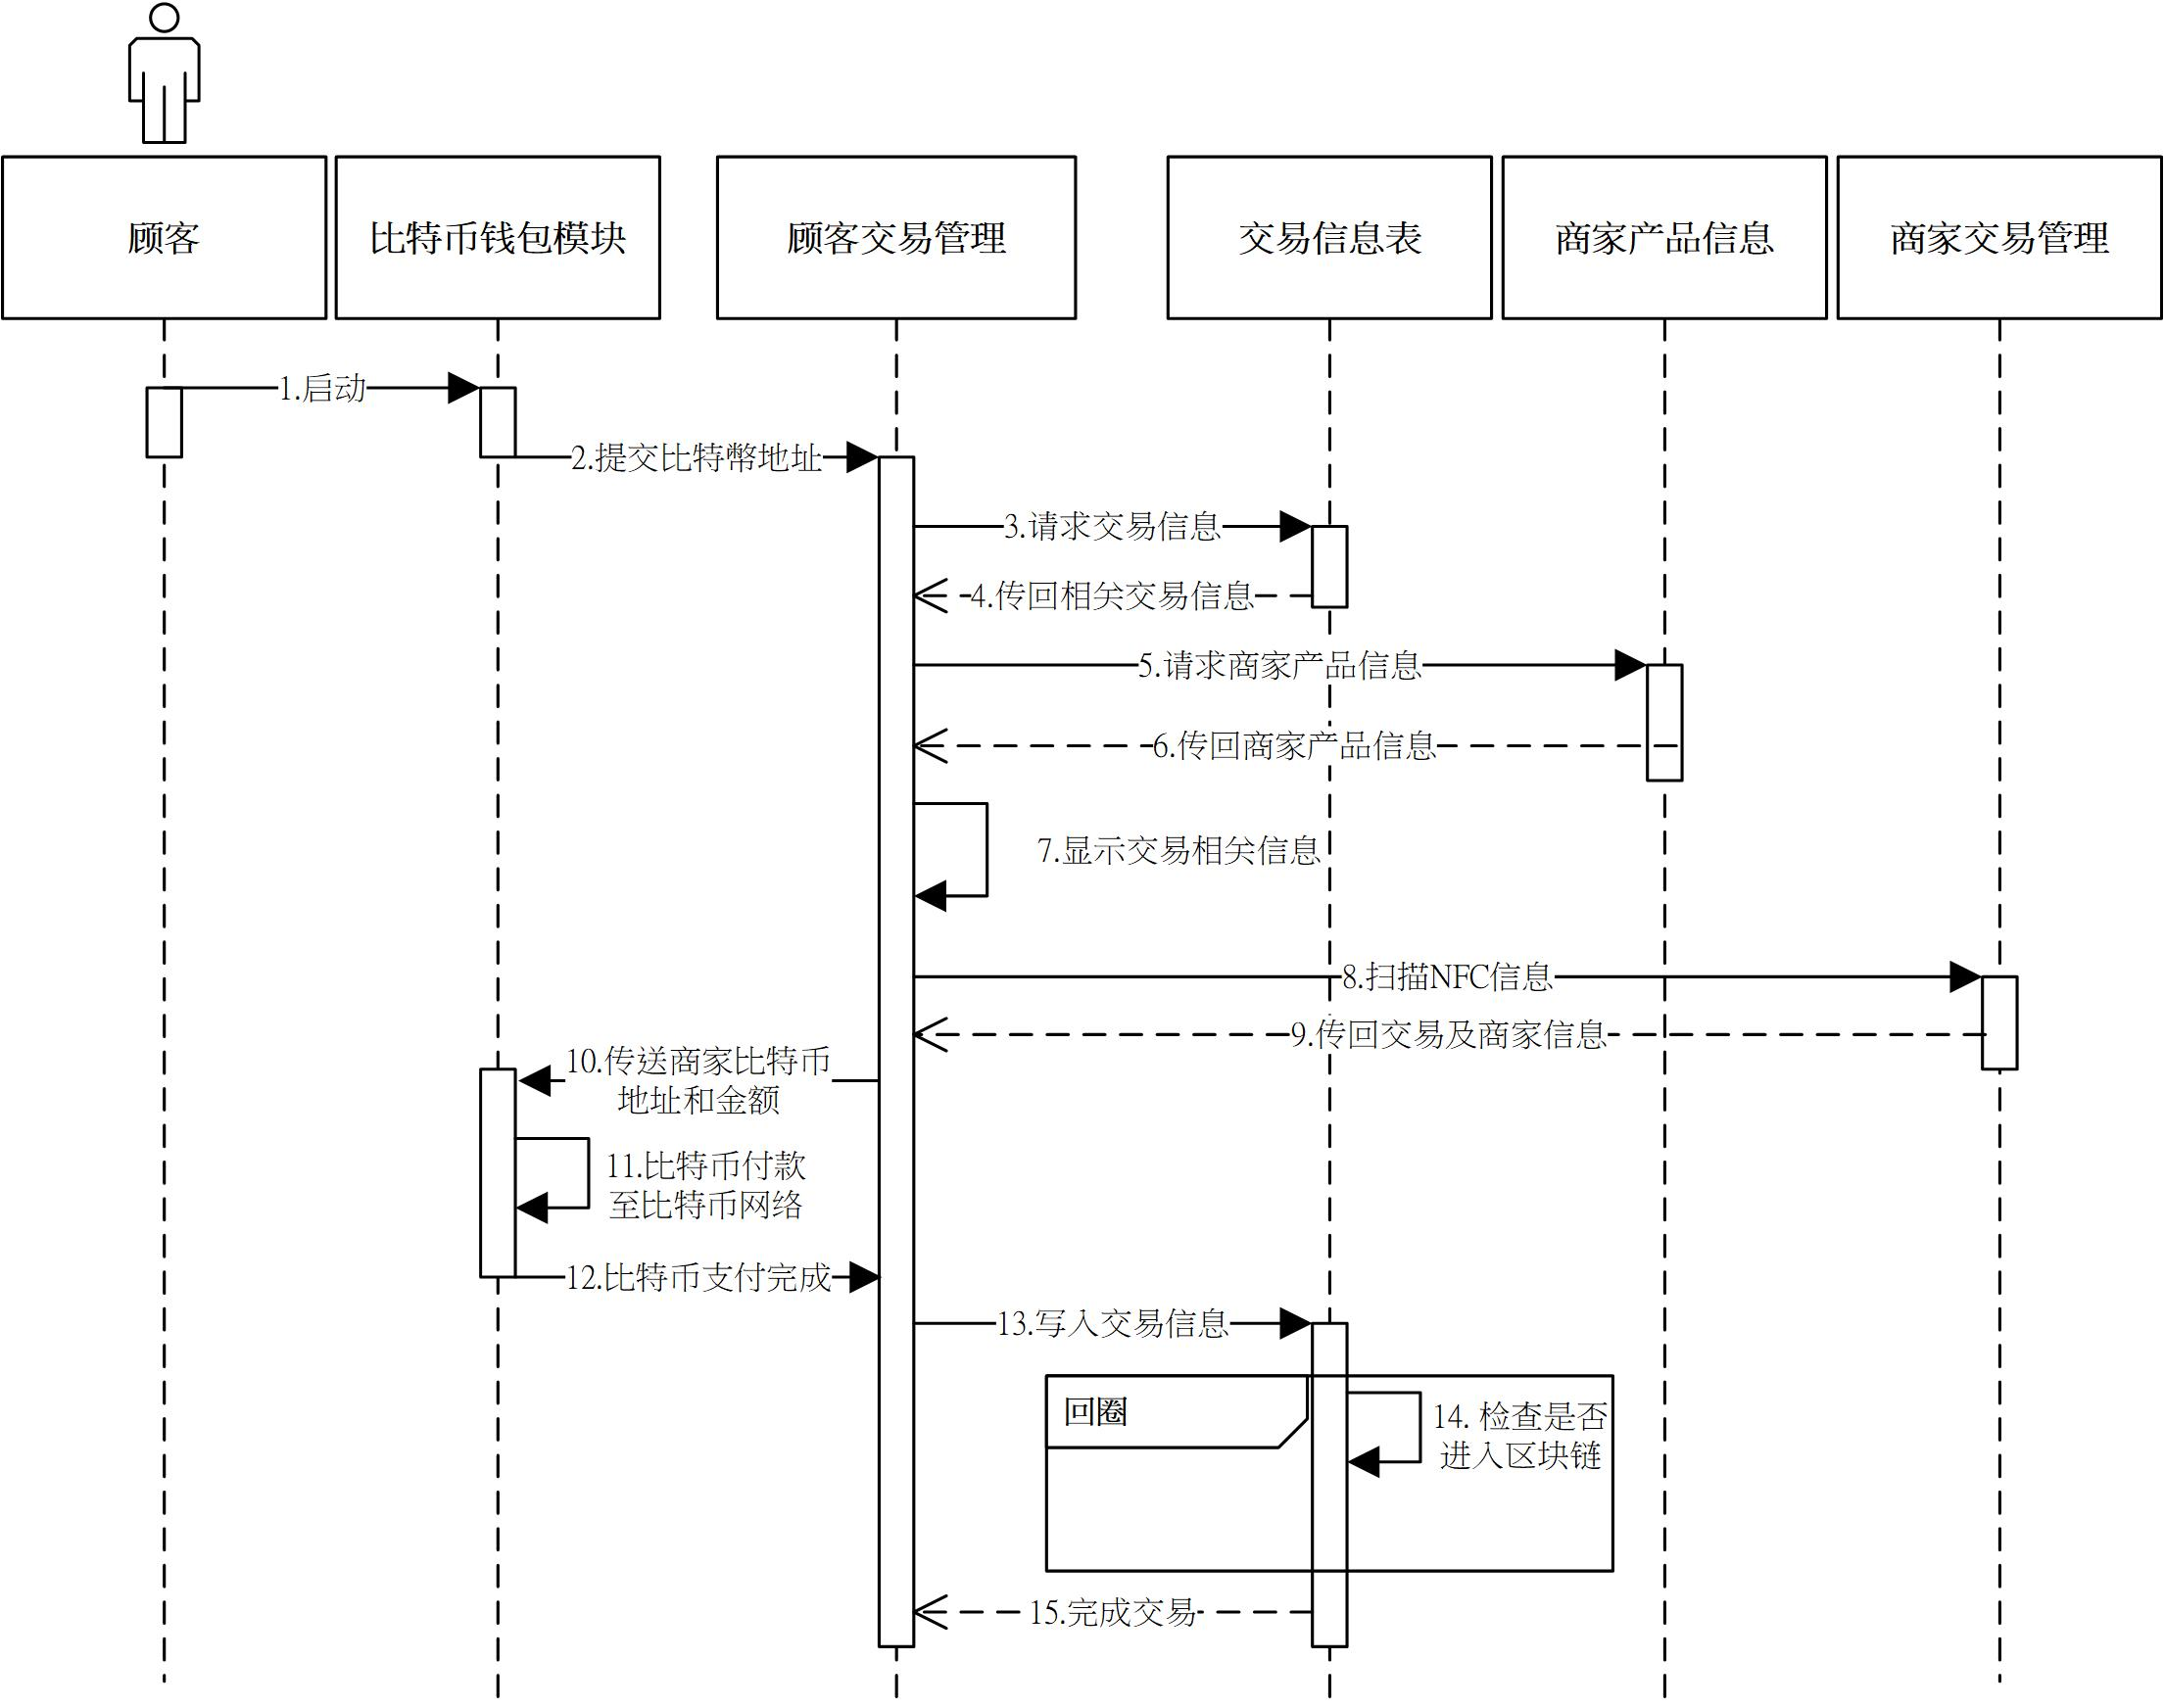
\includegraphics[width = 1\textwidth]{time5.jpg}
		\caption{顧客交易管理時序圖}\label{time5}
	\end{figure}

	\begin{figure}[htbp]
		\centering
		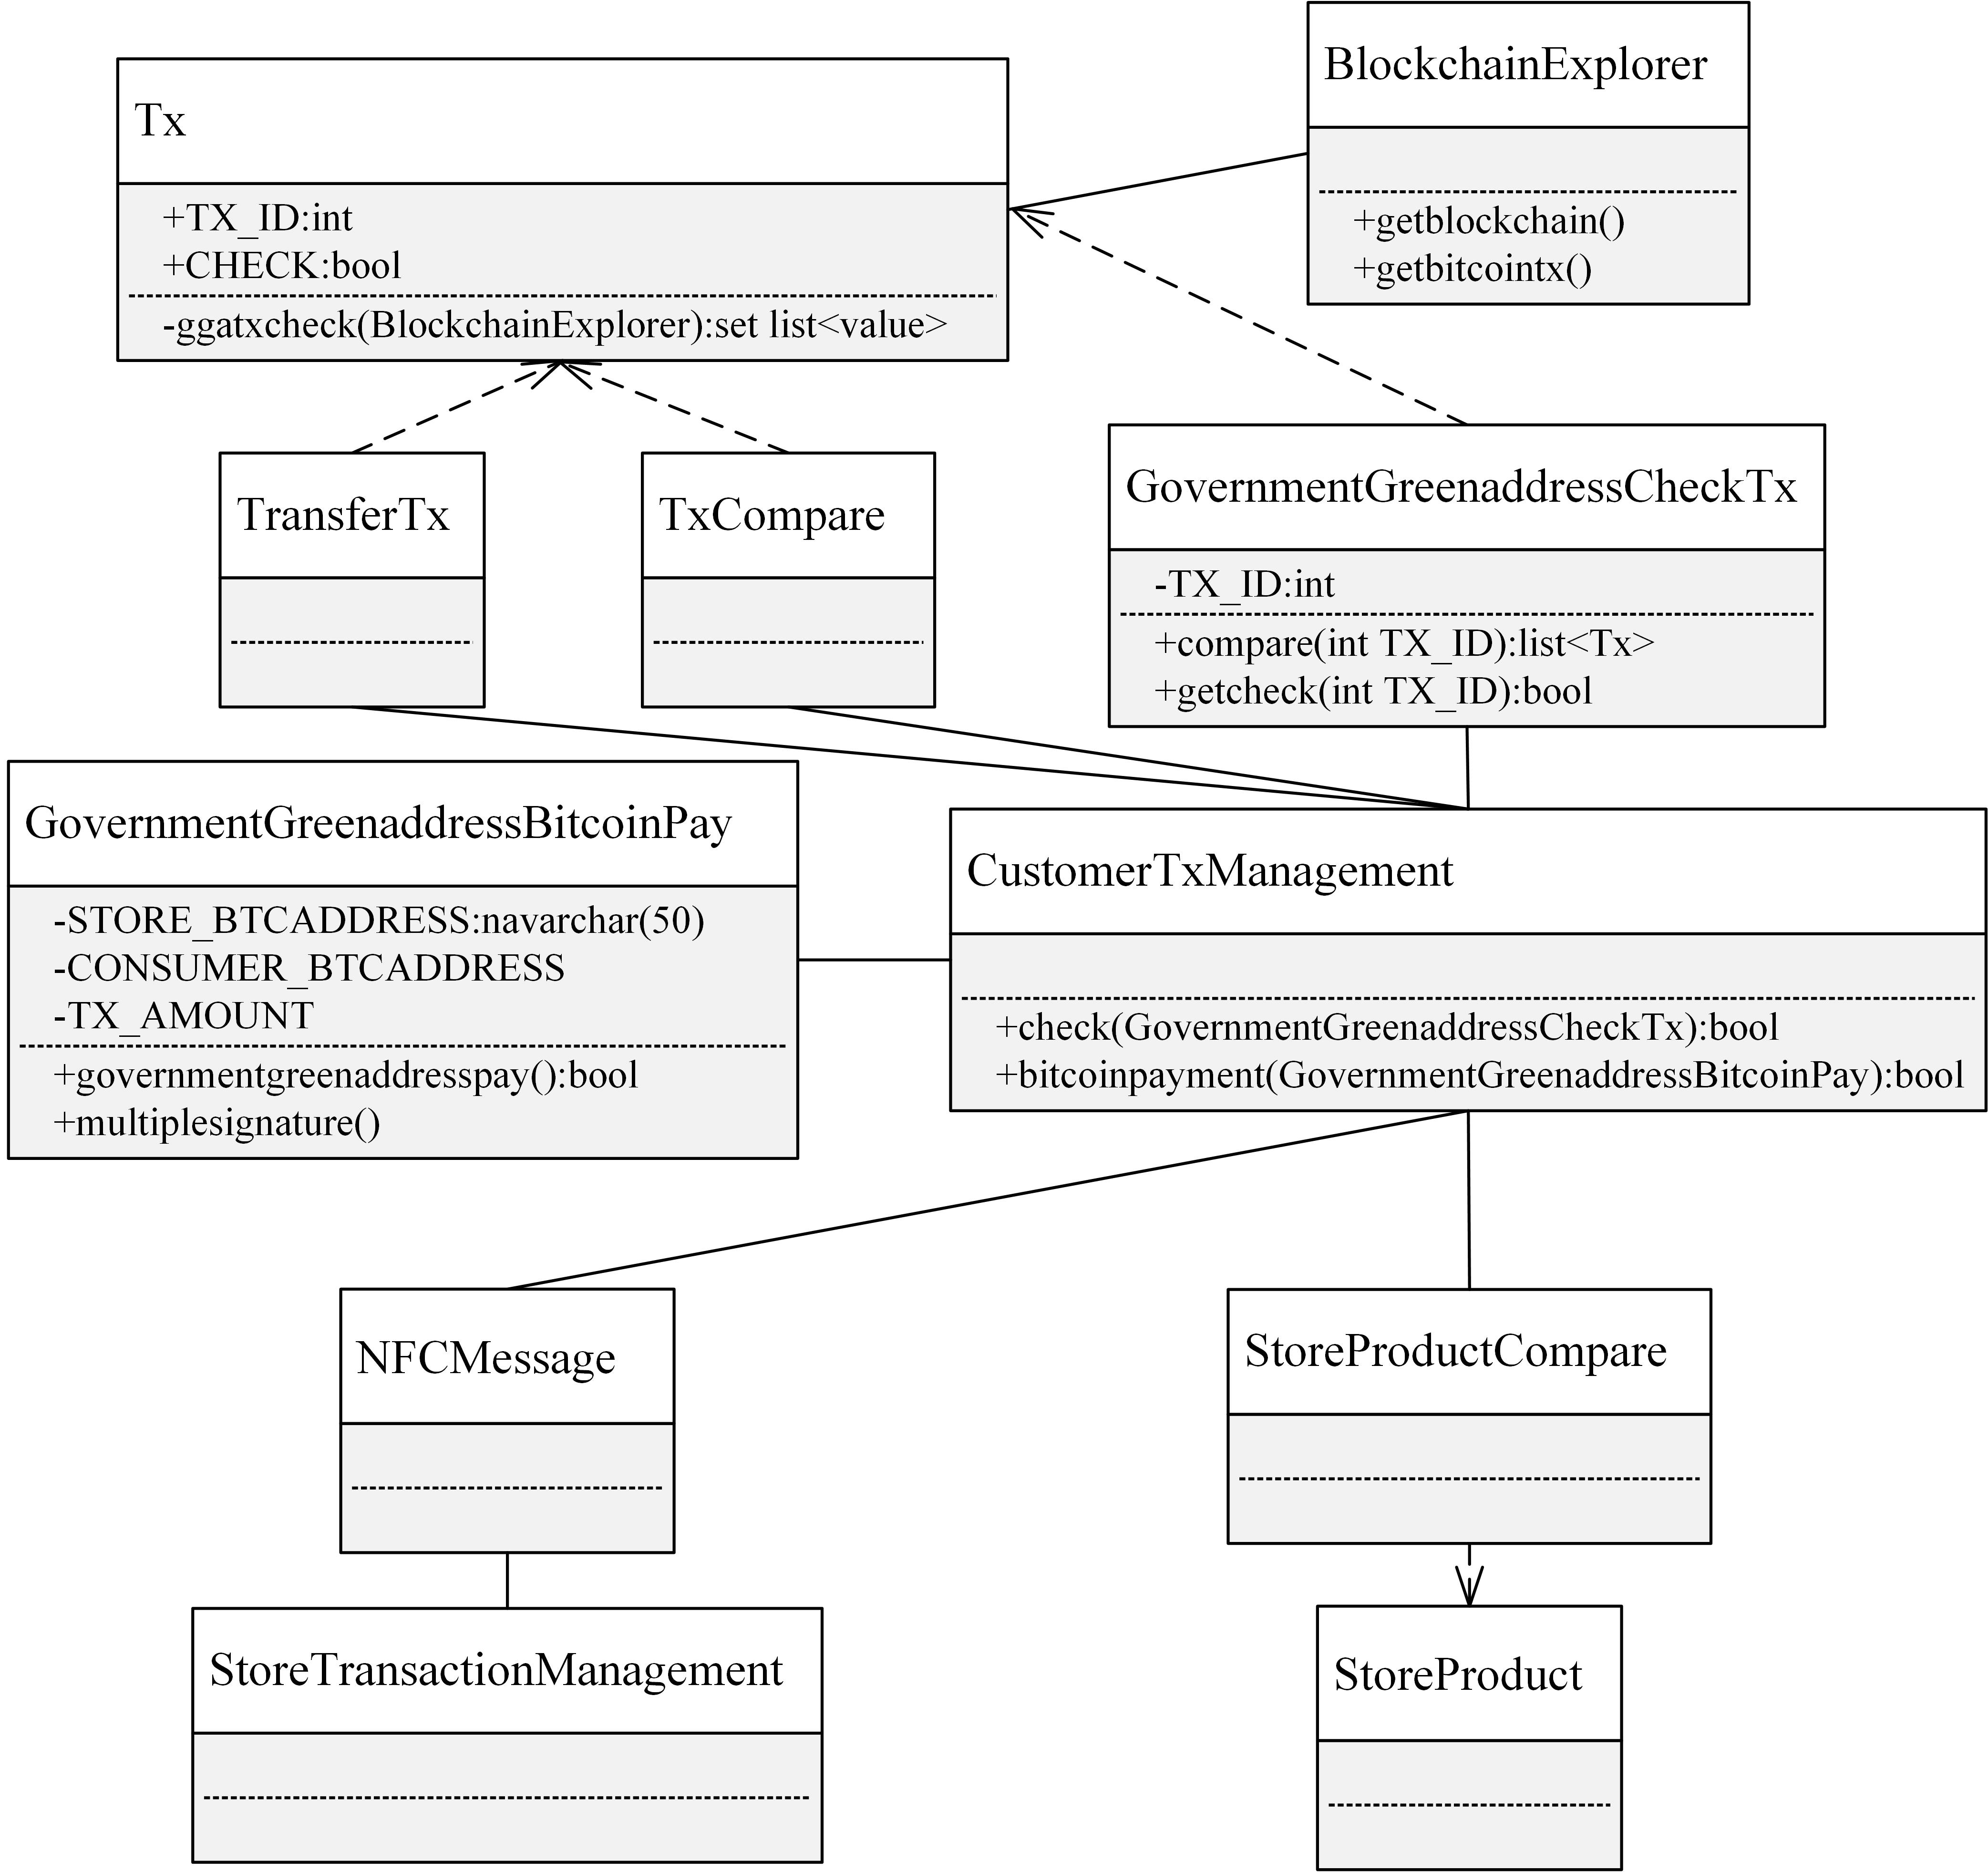
\includegraphics[width = 0.8\textwidth]{c6.jpg}
		\caption{顧客交易管理GA模塊類圖}\label{c6}
	\end{figure}



	\begin{enumerate}
	\item
	\end{enumerate}


\subsubsection{(五)商家交易管理模塊}

	\begin{figure}[htbp]
		\centering
		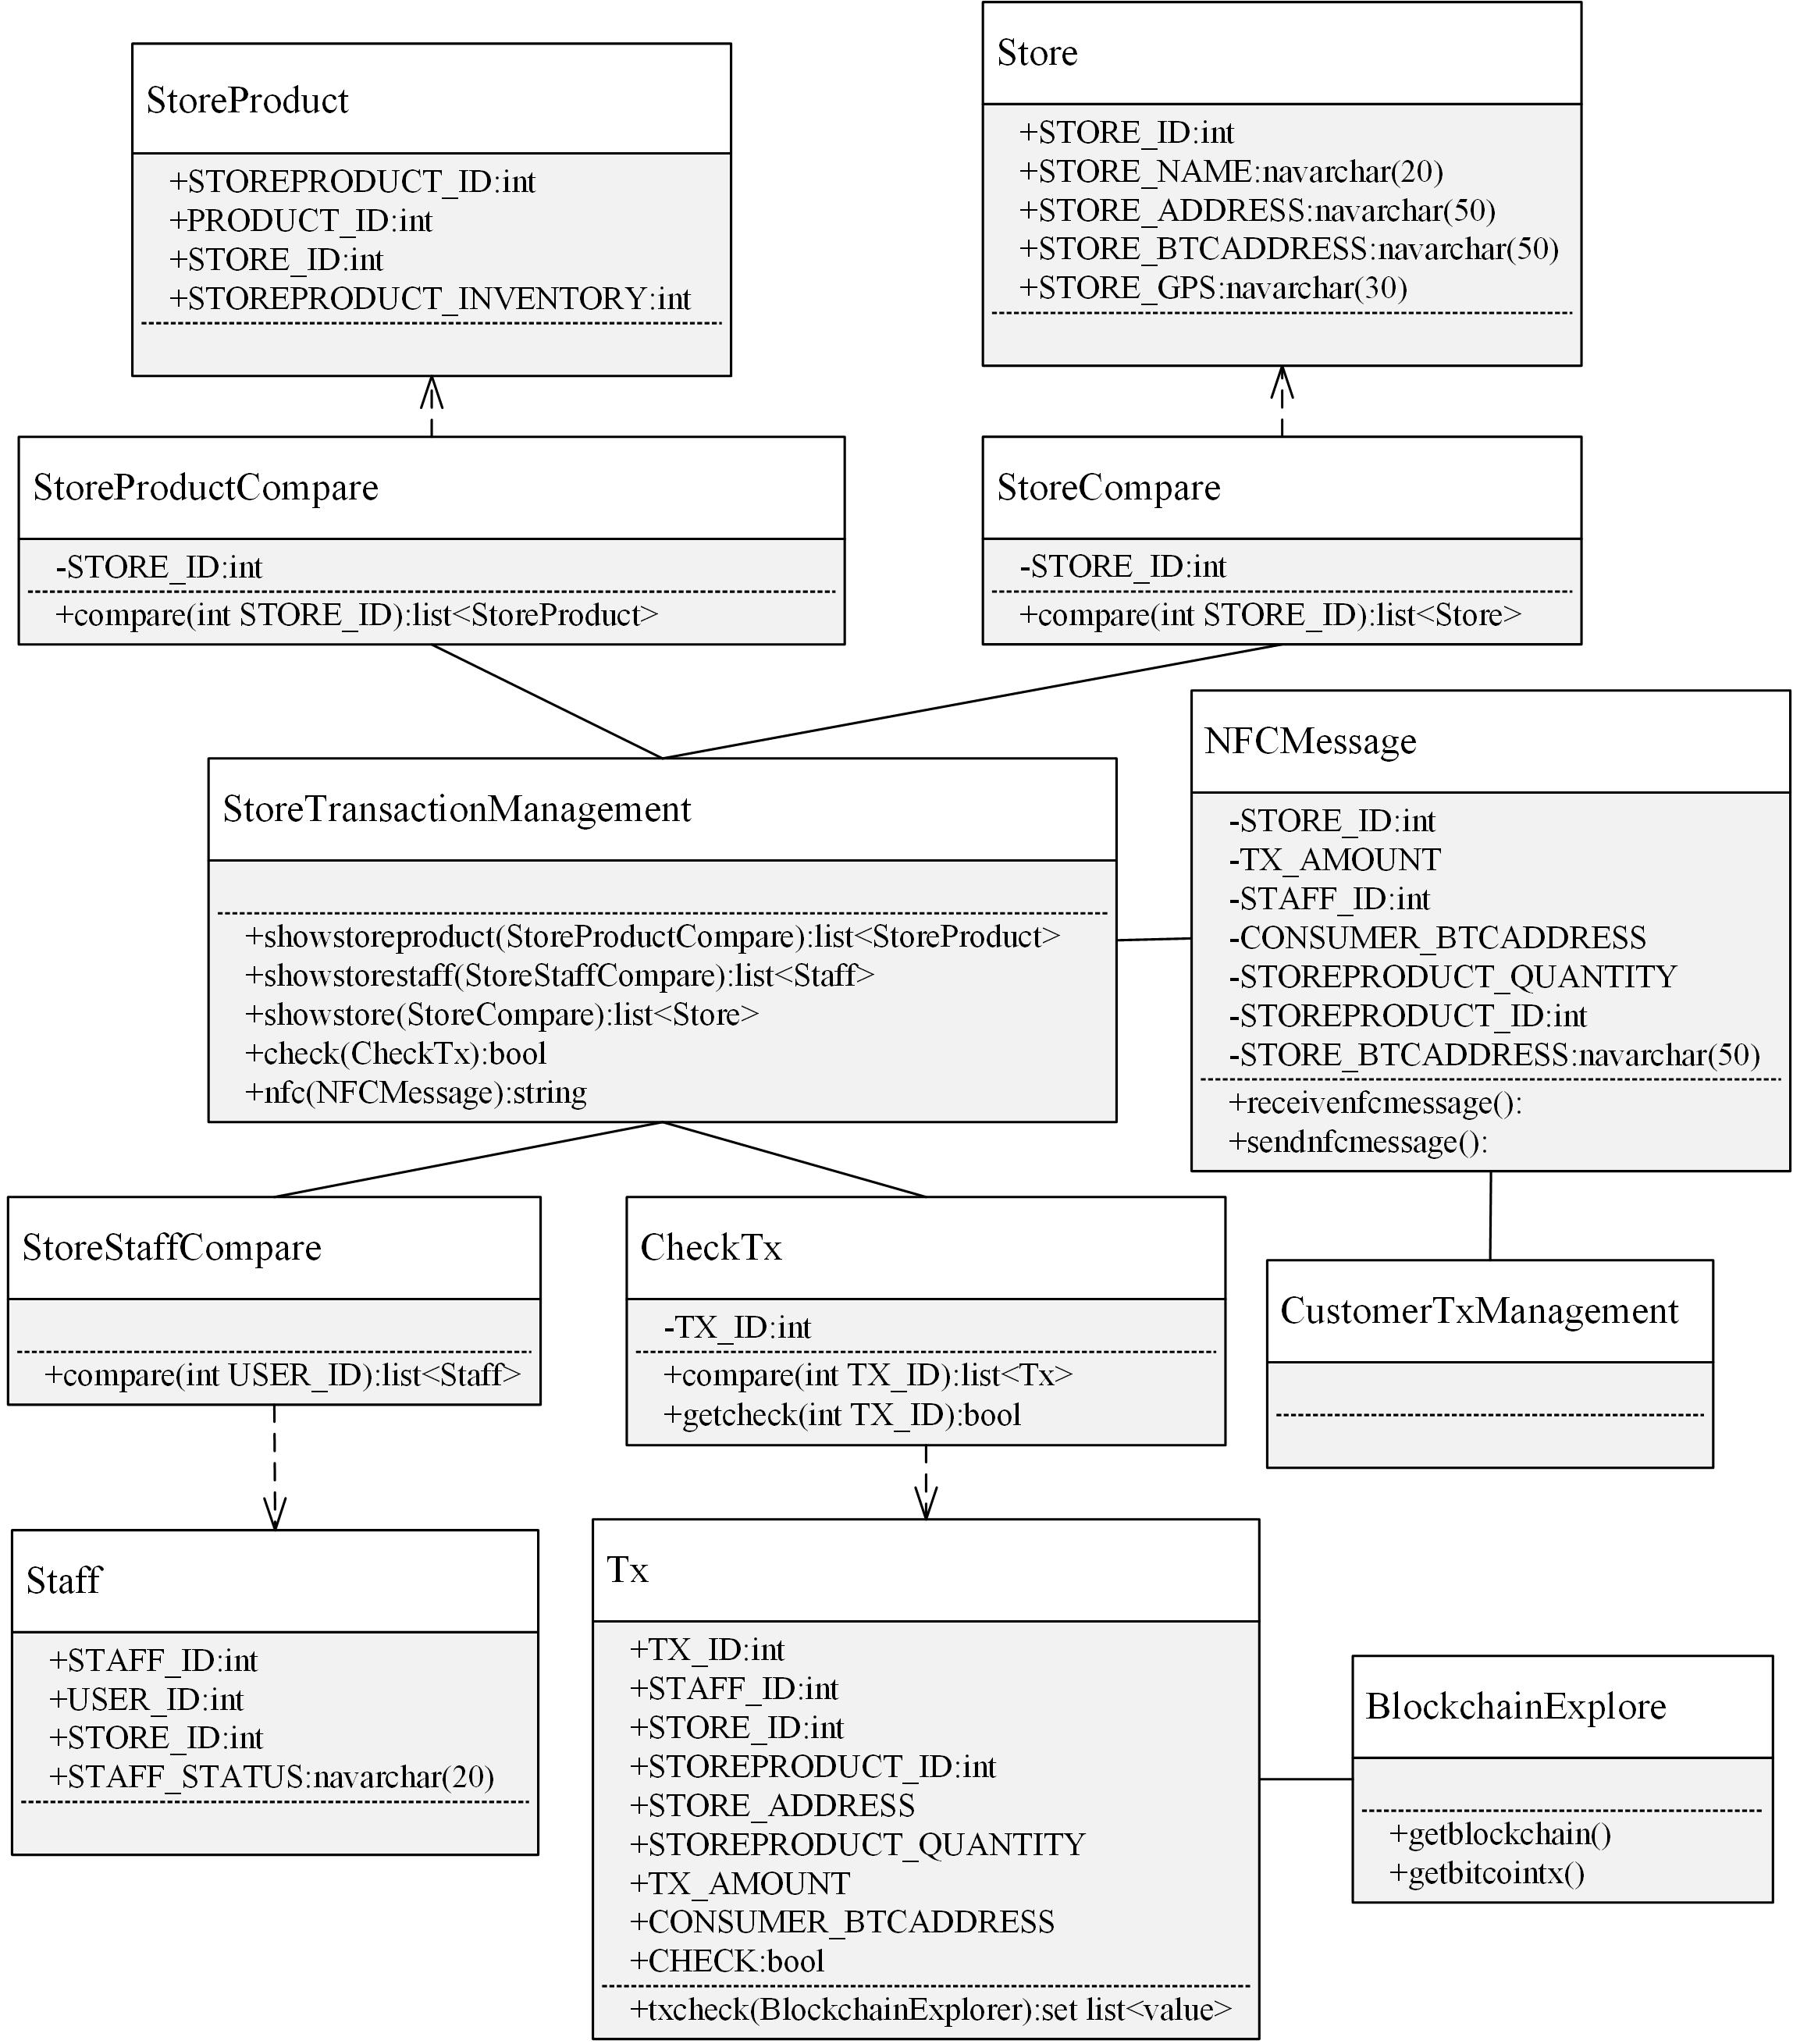
\includegraphics[width = 1\textwidth]{c5.jpg}
		\caption{商家交易管理模塊類圖}\label{c5}
	\end{figure}

圖\ref{time4}

	\begin{figure}[htbp]
		\centering
		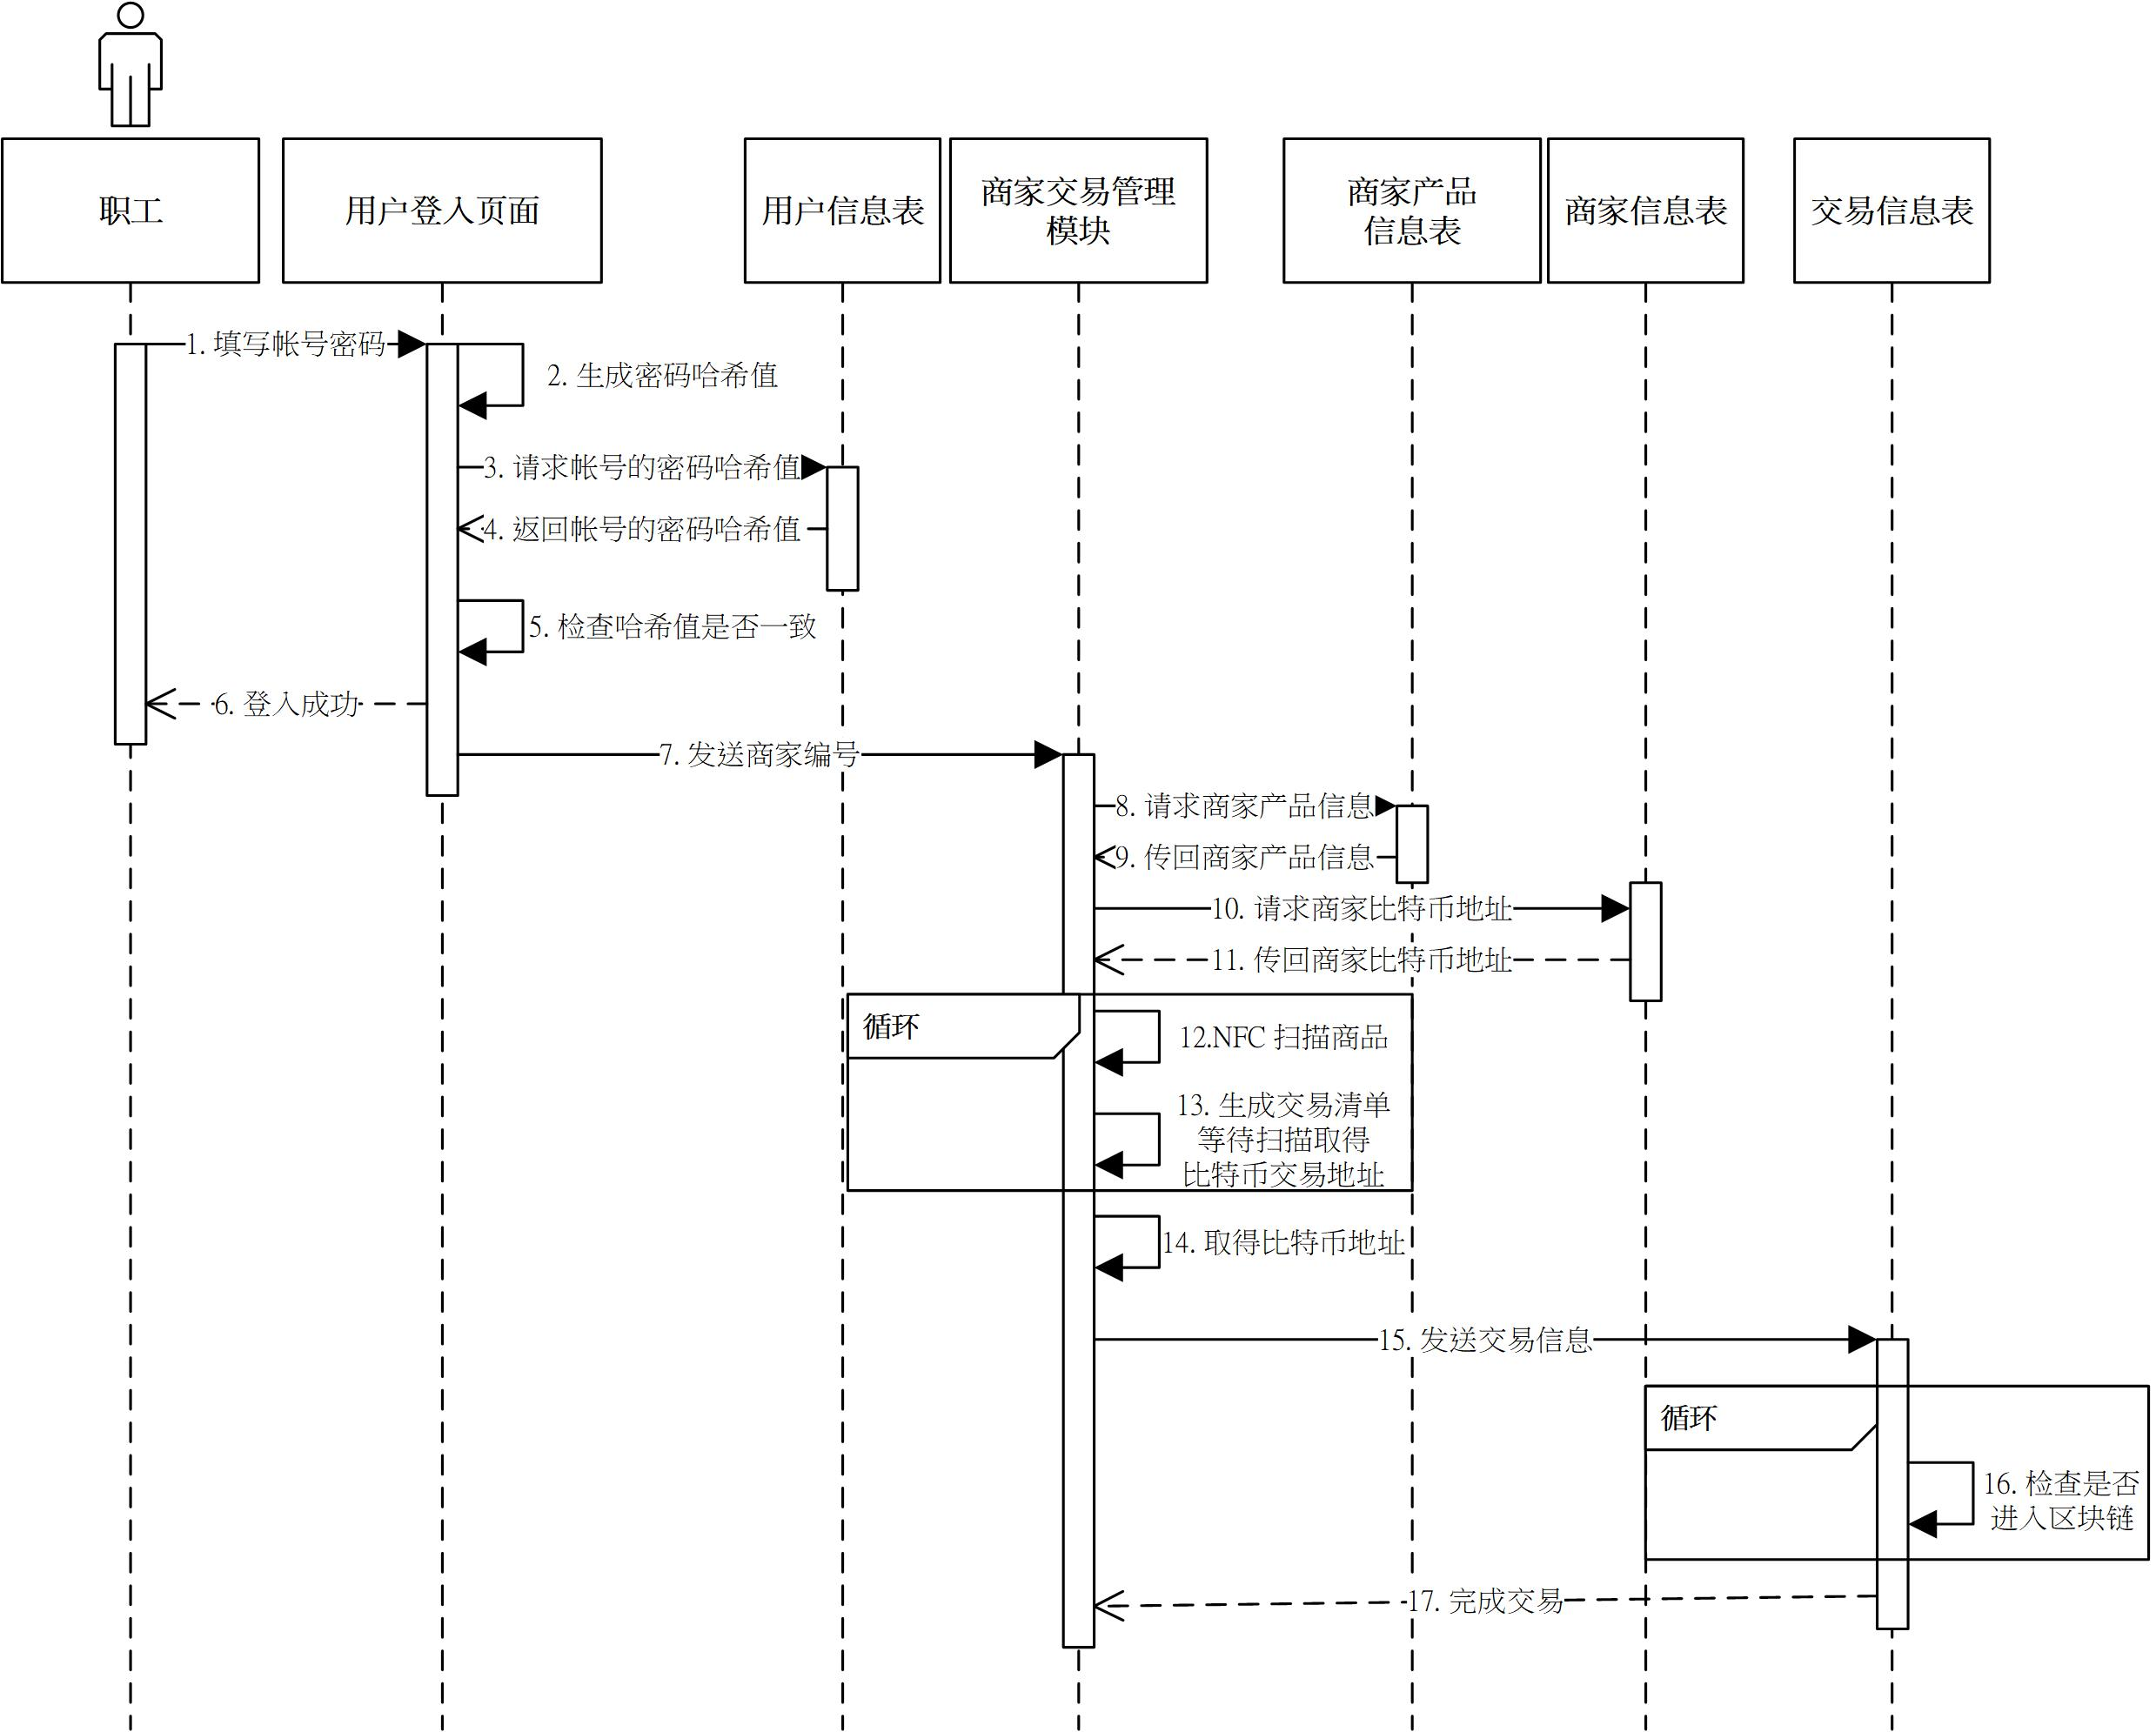
\includegraphics[width = 1\textwidth]{time4.jpg}
		\caption{商家交易管理時序圖}\label{time4}
	\end{figure}

	流程說明:

	\begin{enumerate}
	\item
	\end{enumerate}

	\begin{figure}[htbp]
		\centering
		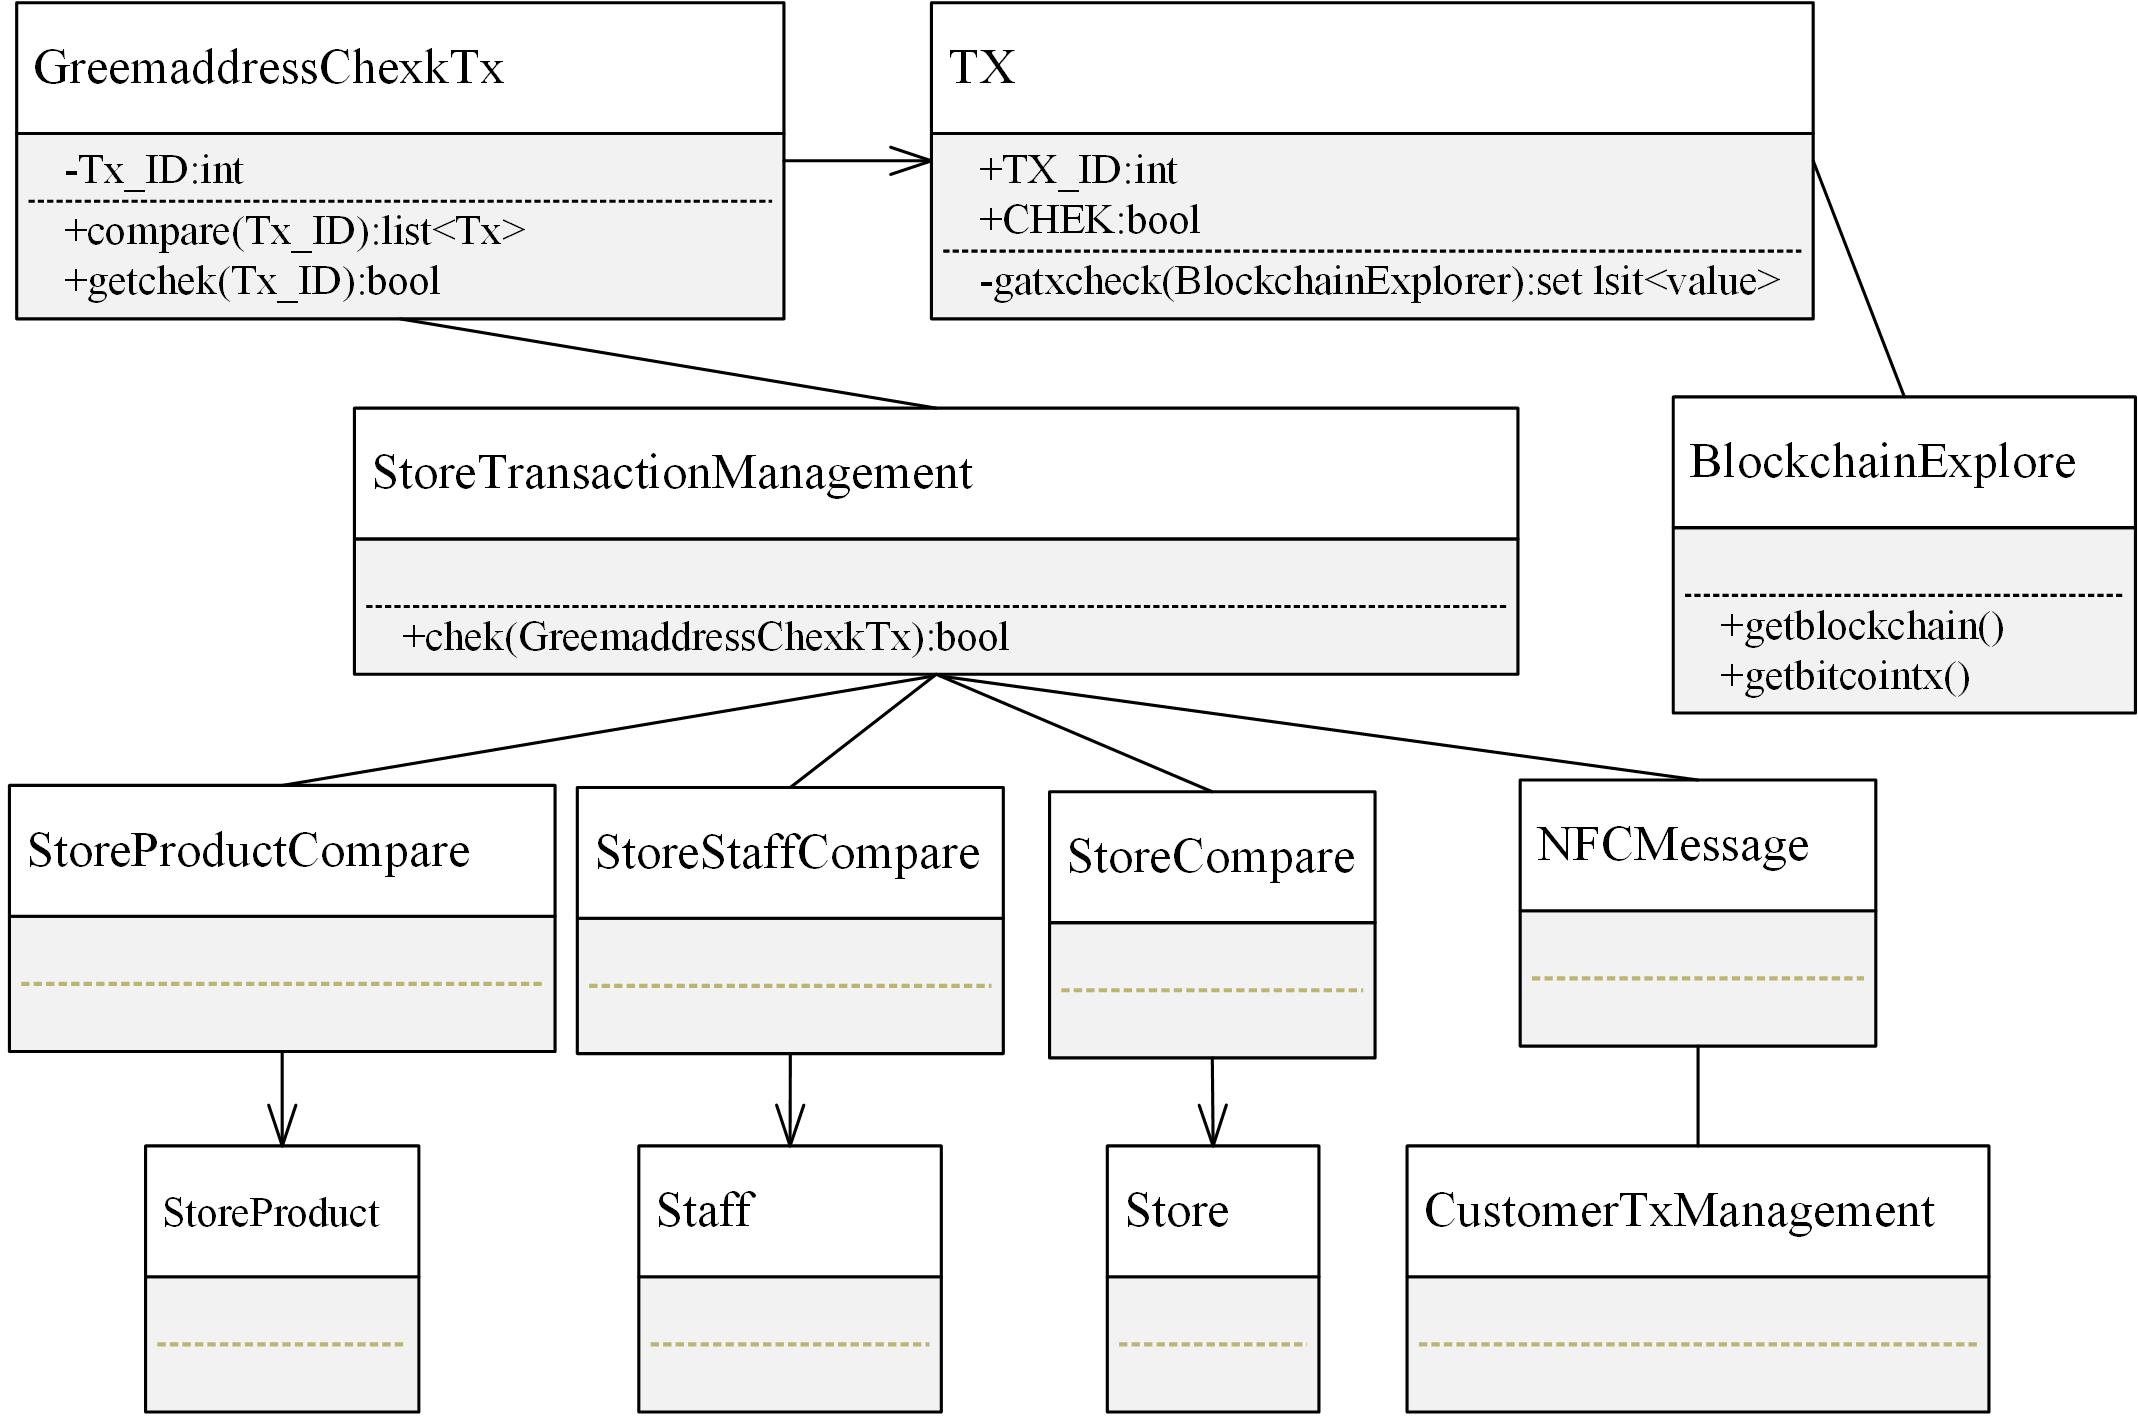
\includegraphics[width = 1\textwidth]{c7.jpg}
		\caption{商家交易管理模塊類圖}\label{c7}
	\end{figure}




\section{系統實現}

% \section{區塊鏈的實名交易監督系統實現}

為了驗證和證明所提議的BRTMS用於比特幣支付收款監督的可行性和有效性,我們將其運行在用於商家商品管理和維護的Java應用程序的SMIMSS子系統,用於商家職工的運行在Android App上的SMCTSS以及運行在App上的用於客戶的CMPTSS。
如圖\ref{fig5}所示,SMIMSS Java應用程序可以幫助商家登錄到系統或創建一個新帳戶。 授權商家成功登錄系統後,商家可以插入或更新產品列表,如圖\ref{fig6}所示。實施的SMIMSS Java應用程序執行前面部分中所述的功能。

\begin{figure}[htbp]
	\centering
	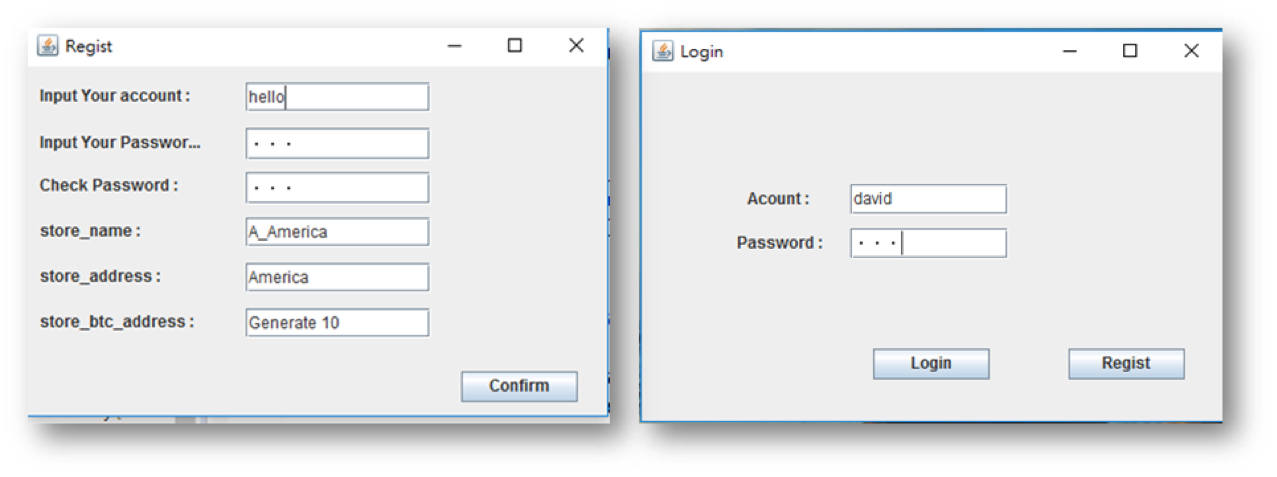
\includegraphics[width = 0.9\textwidth]{fig5.png}
	\caption{SMIMSS的Java應用程序的註冊和登錄界面}\label{fig5}
\end{figure}

\begin{figure}[htbp]
	\centering
	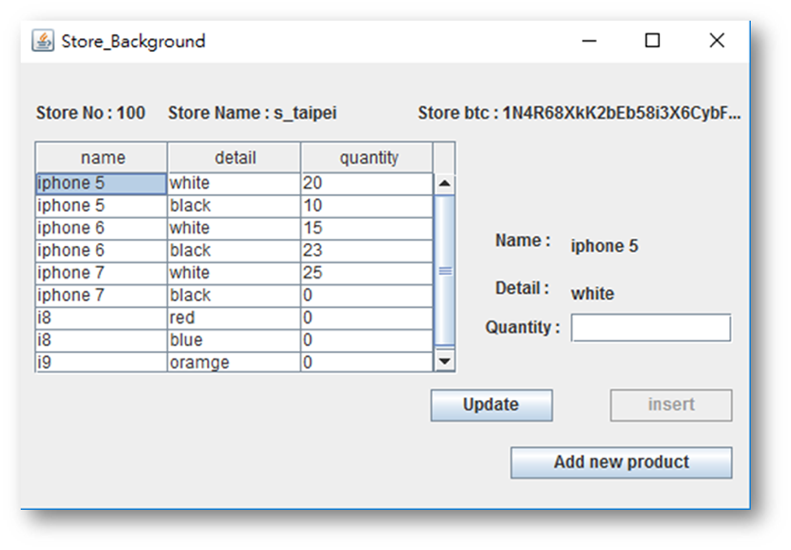
\includegraphics[width = 0.6\textwidth]{fig6.png}
	\caption{在SMIMSS中插入或更新授權商家的產品目錄}\label{fig6}
\end{figure}

商家的產品信息可以通過RFID標籤掃描,存儲到雲端數據庫中,商家職工可以使用我們實現的SMCTSS Android客戶端,啟用NFC監聽器,從購物車中的客戶購買產品中讀取RFID標籤信息。 在如圖\ref{fig7}所示的第一項活動中,商家職工必須登錄才能獲得授權訪問SMCTSS功能。 然後,在第二項活動中,SMCTSS應用程序可以通過使用SMIMSS中應用的雲數據庫檢查產品RFID標籤信息並將其展示給客戶,從而將掃描的產品列入購物車。 在圖\ref{fig7}的第三項活動中,顧客可以要求職工取消購買物品以確認最終購買。 最後,SMCTSS應用程序將自動使用比特幣測試網絡(Bitcoin Testnet)\supercite{bitcointestnet}幫助職工確認發布此加密貨幣交易的收款人地址,如圖\ref{fig7}所示。    

\begin{figure}[htbp]
	\centering
	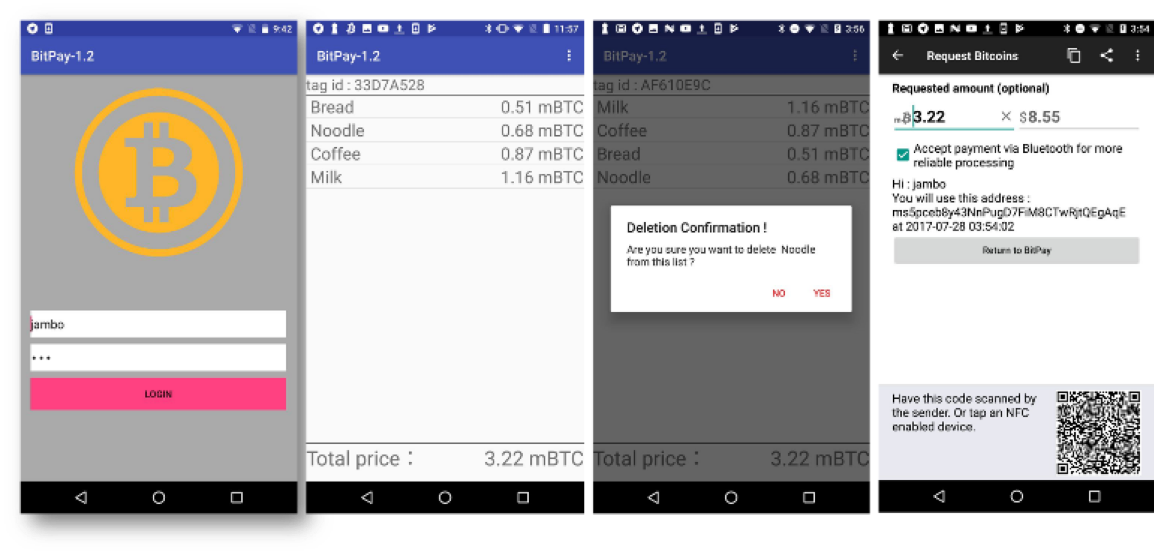
\includegraphics[width = 1\textwidth]{fig7.png}
	\caption{登錄、等待結帳的商品、刪除商品及支付確認}\label{fig7}
\end{figure}

同時,客戶將使用與SMCTSS App相對應的CMPTSS Android App通過比特幣加密貨幣完成採購產品交易。 如圖\ref{fig8}所示,第一個活動表示顧客確認購買產品創建交易數據庫的交易清單,第二個活動顯示包括金額和付款人比特幣地址在內的付款確認,第三個活動顯示交易歷史記錄 的交易作為買方甚至是賣方,最後在第四項活動中顯示了該筆交易詳細採購產品的發票。    

\begin{figure}[htbp]
	\centering
	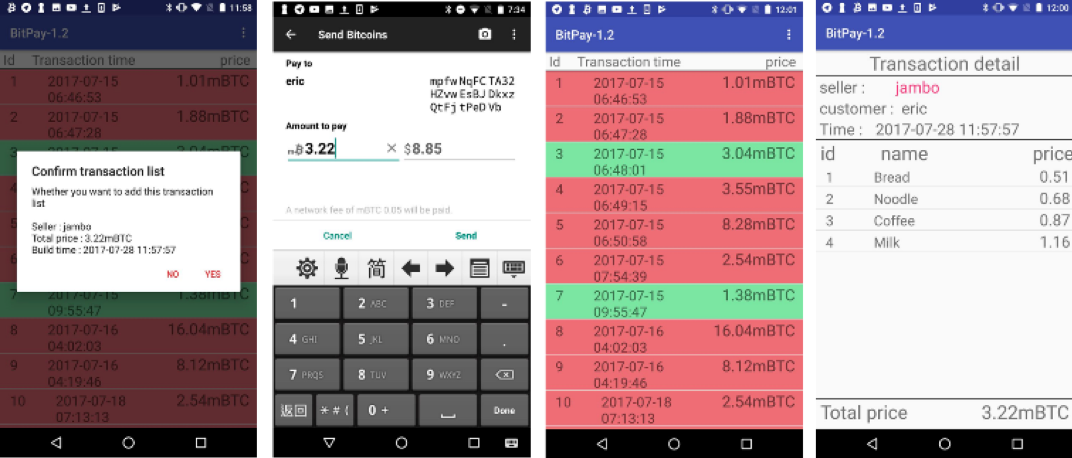
\includegraphics[width = 1\textwidth]{fig8.png}
	\caption{在CMPTSS App中,交易確認,付款確認、交易歷史記錄和發票}\label{fig8}
\end{figure}